\documentclass[11pt]{amsart}

%% ====================================================================
% STYLE / FONTS
%% ====================================================================
\usepackage{eulervm}
\usepackage{eufrak}

\usepackage[usenames,dvipsnames,svgnames,table]{xcolor}
\usepackage{amssymb,amsfonts}
\usepackage{amsmath,amsthm}
\usepackage{pgf, tikz}
\usetikzlibrary{arrows.meta, positioning, shapes.geometric, calc, decorations.pathreplacing, backgrounds, fit}
\usepackage{enumitem}
\usepackage{graphicx}
\usepackage{booktabs}
\usepackage{dsfont}
\usepackage[pdfdisplaydoctitle,colorlinks,urlcolor=blue,linkcolor=blue,citecolor=blue]{hyperref}
\usepackage{xurl}
\usepackage{algorithm}
\usepackage{algorithmic}
\usepackage{multirow}
\usepackage{caption}
\usepackage{subcaption}
\usepackage{colortbl}

\setlength{\textwidth}{15cm}
\setlength{\oddsidemargin}{0cm}
\setlength{\evensidemargin}{0cm}
\setlength{\topmargin}{0cm}
\setlength{\textheight}{22cm}
\emergencystretch=2em

\renewcommand{\rmdefault}{ppl}
\renewcommand{\sfdefault}{fvs}
\renewcommand{\ttdefault}{fvm}

%% ====================================================================
% MACROS
%% ====================================================================
\newcommand{\dd}{\,{\rm d}}
\newcommand{\argmax}{\,{\rm argmax}}
\newcommand{\argmin}{\,{\rm argmin}}
\newcommand{\e}{\epsilon}
\renewcommand{\d}{\delta}
\renewcommand{\a}{\alpha}
\renewcommand{\b}{\beta}
\newcommand{\g}{\gamma}
\newcommand{\p}{\partial}

\newcommand\R{{\mathbb{R}}}
\newcommand\1{{\mathds{1}}}
\newcommand\PP{{\mathbb{P}}}
\newcommand\E{{\mathbb{E}}}
\newcommand\N{{\mathbb{N}}}
\newcommand\A{{\mathcal{A}}}
\newcommand\C{{\mathcal{C}}}
\newcommand\F{{\mathcal{F}}}
\newcommand\V{{\mathcal{V}}}
\newcommand\G{{\mathcal{G}}}

%% ====================================================================
% THEOREMS
%% ====================================================================
\newtheorem{theorem}{Theorem}[section]
\newtheorem{proposition}[theorem]{Proposition}
\newtheorem{lemma}[theorem]{Lemma}
\newtheorem{corollary}[theorem]{Corollary}
\theoremstyle{definition}
\newtheorem{definition}[theorem]{Definition}
\newtheorem{assumption}[theorem]{Assumption}
\theoremstyle{remark}
\newtheorem{remark}[theorem]{Remark}
\newtheorem{observation}[theorem]{Observation}
\numberwithin{equation}{section}

\begin{document}

\title[When Does Multi-Agent Architecture Matter?]
{When Does Multi-Agent Architecture Matter?\\[3pt]
A Falsification Study of Six Interventions\\[2pt]
and the Verifiability Boundary}

\author{Charafeddine Mouzouni}

\address{OPIT -- Open Institute of Technology, and Cohorte AI, Paris, France.}
\email{charafeddine{@}cohorte.co}
\dedicatory{\small\textit{OPIT -- Open Institute of Technology, and Cohorte AI, Paris, France.}\\[2pt]\texttt{charafeddine@cohorte.co}}

\date{April 2026}

%% ====================================================================
% ABSTRACT
%% ====================================================================
\begin{abstract}
We investigate when multi-agent LLM architecture matters for reasoning tasks.
The short answer: on standard text-output benchmarks with a capable proposer, it does not---and with a weak proposer, it actively hurts.
An LLM synthesis node that reads $K$ candidate answers and selects the best one produces \textbf{negligible gains} over simple majority vote across three benchmarks at $n\!=\!1{,}000$: MMLU-Pro ($-1.1$pp), ARC-Challenge ($-1.0$pp), and MATH-500 ($+1.2$pp at $n\!=\!500$), none statistically significant.
With a weaker proposer model, the same synthesizer \textbf{reduces} correctness by $-4.8$pp on MATH-500---the noisy candidate pool misleads the aggregator.
On \textbf{visual-spatial structured output} (ARC-AGI), the synthesizer hurts dramatically ($-13$ to $-20$pp) regardless of proposer quality.
We term this the \emph{verifiability boundary}: a modality threshold (text: neutral; structured visual: harmful) combined with a proposer-quality interaction (weak proposals: harmful even on text tasks).

Replacing the LLM aggregator with a \textbf{symbolic verifier} (sandboxed Python execution) is the only intervention that moves the needle.
On three benchmarks with $K\!=\!16$ independent samples from a $22$B-parameter model, execution-based filtering, and majority vote:
AIME~2024+2025 $40/60 = 66.7\%$ (within $4$pp of a same-task o4-mini reasoning baseline at $2.2\times$ lower cost);
ARC-AGI-1 $73/400 = 18.2\%$ (lowest cost-per-correct in our comparison);
HumanEval $97.0\%$ pass@$16$ (tying a same-metric gpt-5.4-mini baseline of $96.3\%$ at $4.3\times$ lower cost).
Five architectural elaborations tested at matched budgets---game-theoretic allocation, critic feedback, sampling scaling, model diversity, evolutionary refinement---all produce null results against the trivial baseline.
These are falsifications of specific implementations on specific benchmarks, not universal impossibility results.

Code and data: \url{https://github.com/Cmouzouni/verifier-is-all-you-need}.
\end{abstract}

\keywords{multi-agent LLMs, falsification, verifiability boundary, symbolic verification, inference-time compute, ARC-AGI, AIME, HumanEval.}

\maketitle

%% ====================================================================
\section{Introduction}\label{sec:intro}
%% ====================================================================

Modern reasoning models---large language models trained or prompted to produce extended chain-of-thought before answering---have become the dominant paradigm for hard inference tasks \cite{Wei2022CoT, Wang2023SelfConsistency}.
Their effectiveness comes at a cost: they generate many \emph{thinking tokens} per query, often consuming $10$--$100\times$ the compute of a direct answer.
For deployment at scale---in tutoring systems, code assistants, scientific copilots, or autonomous agents---this serial-depth approach is economically prohibitive.

This paper investigates a structurally different alternative.
Instead of one expensive model that thinks for a long time, we use \emph{many cheap models that interact}.
The agents are coordinated by a graph-constrained protocol that distributes them across distinct reasoning frameworks and aggregates their outputs through an explicit synthesis stage.
We initially conjectured that a game-theoretic congestion mechanism---inspired by mean-field-game models of population control \cite{LasryLions2007, HuangMalhameCaines2006, Gomes2010}---would be the active ingredient: agents would be pushed away from crowded frameworks, the population would diversify, and synthesis would aggregate the diverse candidates into a correct final answer.
Our experiments falsify this conjecture cleanly: the congestion mechanism produces diversification as predicted, but the diversification does not translate into correctness gains because the synthesis stage is robust to the framework distribution. The dominant lever is the architectural choice to include a synthesizer at all---not the statistical structure of how agents are distributed.

\paragraph{The central question.}
We ask: \emph{does multi-agent LLM architecture---the choice of how to allocate, aggregate, critique, and iterate over candidate solutions---produce detectable improvements on reasoning tasks?}

Our findings are precise and, we believe, clarifying.
On three standard text-output benchmarks at $n\!=\!1{,}000$ (MMLU-Pro $-1.1$pp, ARC-Challenge $-1.0$pp) and $n\!=\!500$ (MATH-500 $+1.2$pp), an LLM synthesis node produces \textbf{no detectable advantage} over simple majority vote (Wilson CIs: $\pm 3$pp at $n\!=\!1{,}000$).
With a weaker proposer (qwen-7b), the same synthesizer \textbf{hurts} by $-4.8$pp on MATH-500---the noisy candidate pool misleads the aggregator.
On \textbf{visual-spatial structured output} (ARC-AGI), the synthesizer hurts dramatically ($-13$ to $-20$pp) regardless of proposer quality.
We term this the \emph{verifiability boundary}: a modality threshold (text output: neutral; structured visual output: harmful) combined with a proposer-quality interaction (weak proposals make the synthesizer counterproductive even on text tasks).

The only lever that moves the needle is \textbf{symbolic verification}: replacing the LLM aggregator with sandboxed Python execution.
On three benchmarks with $K\!=\!16$ independent samples and execution-based filtering: AIME~2024+2025 $40/60 = 66.7\%$ (within $4$pp of a same-task o4-mini baseline at $2.2\times$ lower cost), ARC-AGI-1 $73/400 = 18.2\%$ (lowest cost-per-correct in our comparison), and HumanEval $97.0\%$ pass@$16$ (tying a same-metric gpt-5.4-mini baseline of $96.3\%$ at $4.3\times$ lower cost).
Five architectural elaborations tested at matched budgets all produce null results against the trivial baseline (Section~\ref{sec:act2-six-nulls}).

\paragraph{Why this matters.}
The multi-agent LLM literature is investing heavily in elaborate wiring: debate protocols \cite{Du2023Debate}, critic-proposer loops \cite{Shinn2023Reflexion, Madaan2023SelfRefine}, game-theoretic routing, and mixture-of-agents layering.
Our results suggest that, at least on the task classes and models we study, this investment does not produce detectable gains.
The engineering effort that does pay off is in the verifier: when candidates can be tested by execution rather than judged by an LLM, the simplest possible architecture ($K$ samples, execution, majority vote) suffices.
Zhang et al.\ \cite{Zhang2025StopOvervaluingMAD} independently reach a similar conclusion for multi-agent debate at matched compute; our work extends their finding to five additional mechanisms, four additional benchmarks, and a systematic gradient across verification regimes.

\paragraph{Approach.}
We organize a population of $N$ deliberating agents on a directed graph $\G = (\V, \mathcal{E})$ whose nodes are externally enforceable protocol states (\textsc{Propose}, \textsc{Critique}, \textsc{Insight}, \textsc{Synthesize}).
Each \textsc{Propose} or \textsc{Insight} agent is assigned to one of $K$ reasoning frameworks via a selection mechanism we vary across experiments (uniform random, deterministic round-robin, or value-aware congestion routing).
The proposers run in parallel and their outputs flow either to a majority-vote aggregator (synthesis-free topologies) or to an LLM \textsc{Synthesize} node that reads all proposals and produces the final answer (synthesis-completed topologies).
The framework selection mechanism is implemented architecturally at the routing decision boundary---not via prompt instructions---in line with prior findings that LLM agents respond to environmental consequences but not to declarative incentives.

\paragraph{Experimental design.}
The empirical campaign totals $\sim\!5{,}650$ episodes and model invocations, organized as: a main sweep ($5$ compositions $\times$ $6$ topologies $\times$ $6$ values of $\g$, $2{,}690$ episodes on a $30$-task battery); four Tier-1 ablations (GSM8K replication, synthesis decomposition, model-family replication, frontier re-baselining); two Tier-2 falsification experiments (MFG vs.\ random vs.\ round-robin, $1{,}350$ episodes); one Tier-3 experiment on ARC-AGI; and the verifiability-gradient experiment on MMLU-Pro, ARC-Challenge, and MATH-500 at $n\!=\!500$--$1{,}000$.
Full experimental details are in Appendix~\ref{app:methods}.

\paragraph{Contributions.}
(1)~We identify the \emph{verifiability boundary}: a two-component criterion (modality threshold $+$ proposer-quality interaction) governing when LLM synthesis helps, is neutral, or hurts.
(2)~We show that replacing the LLM aggregator with a symbolic verifier (sandboxed Python execution) dissolves the boundary, achieving frontier-competitive results on ARC-AGI-1, AIME, and HumanEval with a $22$B model.
(3)~Five architectural elaborations (game-theoretic allocation, critic feedback, sampling scaling, model diversity, evolutionary refinement) all produce null results against the trivial verifier-loop baseline at matched budgets.
(4)~We identify a capability ceiling: the synthesis mechanism saturates at the per-agent recognition ceiling and is counterproductive on strong base models.
Section~\ref{sec:decision-tree} translates these findings into a practical deployment criterion.

%% ====================================================================
\section{Related Work}\label{sec:related}
%% ====================================================================

\paragraph{Reasoning models and inference-time compute.}
The current dominant paradigm for hard reasoning is inference-time scaling: chain-of-thought \cite{Wei2022CoT}, self-consistency sampling \cite{Wang2023SelfConsistency}, best-of-$N$ reranking, and tree-of-thought search \cite{Yao2023ToT} all expand the inference-time compute budget per query.
The trend culminated in dedicated reasoning models that produce hundreds of thinking tokens per query.
These methods are effective but expensive, and the cost grows roughly linearly with the number of generated tokens.
Our work asks whether the same compute budget, redistributed across many small models that interact, can produce better outputs.

\paragraph{Multi-agent LLM systems.}
Multi-agent collaboration frameworks \cite{Wu2023AutoGen, Hong2024MetaGPT, Li2023CAMEL, Qian2024ChatDev}, debate-based reasoning \cite{Irving2018Debate, Du2023Debate, Khan2024Debate}, graph-structured reasoning \cite{Yao2023ToT, Besta2024GoT}, and iterative self-refinement \cite{Shinn2023Reflexion, Madaan2023SelfRefine} represent the empirical landscape that our framework formalizes.
A consistent finding across this literature is that naive scaling of multi-agent systems---more agents, more interaction rounds---does not automatically improve quality, and can amplify failure modes through herding and false consensus.
Our framework explains \emph{when} structured deliberation adds value and \emph{when} it does not, by distinguishing tasks where the population can reach a consensus on the correct answer (the synthesis node has something to work with) from tasks where it cannot.
The capability-ceiling boundary we report is, to our knowledge, the first explicit characterization of when multi-agent deliberation \emph{stops} adding value to a strong base model.

\paragraph{Mean-field games and population control.}
The mean-field game framework \cite{LasryLions2007, HuangMalhameCaines2006} models strategic interaction in large populations through coupled forward--backward systems.
Finite-state MFGs \cite{Gomes2010, Gueant2015, Cecchin2019} reduce the problem to coupled ODEs on the simplex, with well-established existence and uniqueness results under Lasry--Lions monotonicity.
The probabilistic framework of \cite{CarmonaDelarue2018} extends the theory to common noise and major-minor player settings.
MFGs with congestion have been applied to traffic routing \cite{Achdou2020MFGTraffic} and crowd dynamics \cite{Lachapelle2011MFGCrowd}.
We adapt this machinery to multi-agent reasoning, where graph nodes are protocol states, congestion penalties prevent herding on a single reasoning frame, and terminal rewards depend on whether the synthesized output is correct.

\paragraph{Heterogeneous populations and routing.}
Mixture-of-experts architectures \cite{Shazeer2017MoE} route inputs through learned subsets of model parameters; speculative decoding \cite{Leviathan2023Speculative} uses a small draft model whose outputs are verified by a large target model.
Both approaches reduce inference cost by allocating the largest models only to the hardest decisions.
Our work shares the underlying philosophy---compute allocation should be adaptive to problem difficulty---but operates at a higher granularity: instead of routing tokens or attention through a learned router, we route reasoning steps through a population-level mechanism.

\paragraph{Program synthesis and verifier-guided search.}
A growing body of work shows that pairing LLM-generated code with external symbolic verifiers dramatically improves reasoning accuracy.
AlphaCode~2 \cite{Li2022AlphaCode} samples up to a million programs per task and filters via test-case execution, reaching the 85th percentile on competitive programming.
FunSearch \cite{RomeraParedes2024FunSearch} evolves LLM-generated programs against a symbolic evaluator, discovering new mathematical lower bounds.
Snell et al.\ \cite{Snell2024ComputeOptimalTTS} show that compute-optimal test-time search with a process reward model is $4\times$ more efficient than best-of-$N$ sampling, and a small model can beat one $14\times$ larger under FLOPs-matched evaluation.
Liu et al.\ \cite{Liu2025Can1BSurpass405B} push this further: a $7$B model with PRM-guided search matches o1 on MATH-500.
For ARC-AGI specifically, every top-performing entry in the 2024 ARC Prize combines LLM program synthesis with symbolic execution against the training pairs \cite{ARCPrize2024Report}: Aky\"urek et al.\ \cite{Akyurek2024TTT} reach $61.9\%$ on the public eval with an $8$B model and test-time training.
Zhang et al.\ \cite{Zhang2025StopOvervaluingMAD} provide a definitive critique of homogeneous multi-agent debate, showing it loses to single-model self-consistency at matched compute on $9$ benchmarks---a finding our verifiability-boundary results independently corroborate.
Our Section~\ref{sec:act2} experiments apply this verifier-guided template to the multi-agent setting, demonstrating that the generator--verifier decomposition is the mechanism that dissolves the boundary identified in Section~\ref{sec:results}.

\paragraph{LLM self-evaluation and the verification gap.}
The verifiability boundary is related to a growing body of work on the limits of LLM self-assessment.
Saunders et al.\ \cite{Saunders2022SelfCritique} show that LLMs are unreliable self-critics when the evaluation task is as hard as the generation task.
Huang et al.\ \cite{Huang2023SelfCorrection} demonstrate that LLMs cannot reliably self-correct their reasoning without external feedback.
Kamoi et al.\ \cite{Kamoi2024SelfEval} find systematic biases in LLM self-evaluation across multiple benchmarks.
Our verifiability boundary can be understood as an architectural consequence of this same phenomenon: LLM-based synthesis fails precisely when the ``verification'' the synthesizer would need to perform is as hard as the original generation problem.
The novel contribution is showing that this failure mode has a clean architectural remedy (symbolic verification) and that the remedy is sufficient---no additional multi-agent structure is needed on top.

%% ====================================================================
\section{Architecture and Notation}\label{sec:arch}
%% ====================================================================

We organize a population of $N$ deliberating agents on a finite directed graph $\G = (\V, \mathcal{E})$ whose nodes represent \emph{externally certifiable protocol states}---not hidden internal reasoning.
Each node enforces a typed output schema (JSON) and a transition validator that checks edge admissibility before allowing movement.
This makes the architecture inspectable and enforceable: the agent is constrained to operate within a public protocol, regardless of what its internal representations look like.
In our experiments, we instantiate four node types (\textsc{Propose}, \textsc{Critique}, \textsc{Insight}, \textsc{Synthesize}) corresponding to four roles, and test six topologies ranging from \textsc{Propose-only} (no synthesis) to \textsc{Insight+Synth} (the cheapest $100\%$ configuration); full topology definitions are in Appendix~\ref{app:methods}.
The fundamental architectural distinction is between topologies with and without an explicit synthesis node: synthesis-free topologies aggregate via majority vote; synthesis-completed topologies pass all outputs to a dedicated synthesizer.

Each \textsc{Propose} or \textsc{Insight} agent is assigned to one of $K$ reasoning frameworks via a selection mechanism we vary across experiments: random uniform, deterministic round-robin, or value-aware congestion routing (a softmax over framework values penalized by current occupancy; see Appendix~\ref{app:methods} for the full specification).
The framework selection is enforced by the controller at the routing decision boundary---the LLM is never asked to ``be diverse,'' it is simply assigned to a specific framework.

\paragraph{A conjecture we falsify.}
We initially conjectured that the value-aware congestion strategy---motivated by mean-field-game models of population control \cite{LasryLions2007, HuangMalhameCaines2006, Gomes2010, Gueant2015}---would improve allocation by pushing agents away from crowded frameworks.
Section~\ref{sec:results-falsification} falsifies this conjecture cleanly: the mechanism produces the predicted diversification but the diversification does not translate into correctness gains.
The congestion parameter is therefore presented as one of three framework-selection strategies tested by the ablation, not as a theoretical contribution.

%% ====================================================================
\section{Experimental Methods}\label{sec:methods}
%% ====================================================================

The empirical campaign comprises a \emph{main sweep} that establishes the topology and $\g$ effects across a full factorial design, plus seven targeted ablation experiments.
Full details of population compositions, topologies, congestion implementation, and metrics are in Appendix~\ref{app:methods}.

\paragraph{Task batteries.}
We use two primary batteries.
\emph{Phase~A} consists of $30$ elementary tasks across four domains (algebra, sequences, logic, word problems), each admitting four named solution frameworks and scored by exact string/numeric match---no LLM judge is involved.
For external validation we use $50$ GSM8K problems \cite{Cobbe2021GSM8K} (fixed seed $42$), MATH-500 \cite{Hendrycks2021MATH}, MMLU-Pro, ARC-Challenge, and ARC-AGI \cite{Chollet2019ARC} (visual-spatial structured output).

\paragraph{Models.}
The main sweep uses the Qwen family exclusively: \texttt{qwen-7b} (Qwen-2.5-7B-Instruct-Turbo, $7$B dense, \$$0.30$/M tokens), \texttt{qwen-22b} (Qwen-3-235B-A22B-Instruct, $22$B active, \$$0.20$/$\$0.60$ per M tokens), and \texttt{qwen-17b} (Qwen-3.5-397B-A17B, $17$B active, \$$0.60$/$\$3.60$ per M tokens).
For family replication we additionally use Llama-3.3-70B and DeepSeek-V3.1, both via Together AI.

\paragraph{Experimental design overview.}
The main sweep is $5$ population compositions $\times$ $6$ topologies $\times$ $6$ values of $\g$, with $15$ episodes per condition ($2{,}690$ episodes total).
Four Tier-1 ablations test boundary conditions: hard-benchmark replication (GSM8K), synthesis decomposition, model-family replication, and frontier-fairness re-run.
Two Tier-2 experiments test MFG vs.\ random vs.\ round-robin framework selection ($1{,}350$ episodes).
One Tier-3 experiment tests the synthesis effect on ARC-AGI ($\sim\!1{,}350$ model invocations).
The combined dataset comprises $\sim\!5{,}650$ episodes.
The verifiability-gradient experiment (Table~\ref{tab:gradient}) adds $n\!=\!1{,}000$ episodes each on MMLU-Pro and ARC-Challenge, plus $n\!=\!500$ on MATH-500 with both strong and weak proposers.

%% ====================================================================
\section{Results --- The Verifiability Boundary}\label{sec:results}
%% ====================================================================

Full results for topology dominance (Phase~A bar chart, $\g$ sweep), GSM8K generalization, the capability ceiling, the Pareto frontier, baselines, and the complete ARC-AGI ranking are in Appendix~\ref{app:full-results}.
Here we present the three findings that define the verifiability boundary.

\subsection{The verifiability gradient}\label{sec:gradient}

To test whether the synthesis advantage tracks verification cost, we measured the synth-vs-majority-vote gap across five benchmark--model combinations spanning different verification regimes and proposer strengths:

\begin{table}[h]
\centering\small
\caption{The verifiability gradient. Synthesis vs.\ majority vote across benchmarks and proposer models ($K\!=\!4$). On standard text-output tasks with a strong proposer, the synthesizer is neutral ($\pm 1$pp). With a weaker proposer or on visual-spatial structured output, it \emph{hurts}. Wilson 95\% CIs shown for $n\!\geq\!500$.}
\label{tab:gradient}
\begin{tabular}{@{}llcccl@{}}
\toprule
Benchmark & Proposer & $n$ & MV & Synth & $\Delta$ \\
\midrule
\multicolumn{6}{l}{\emph{Standard text-output tasks}} \\
MMLU-Pro & \texttt{qwen-22b} & $1{,}000$ & $70.8\%$ {\scriptsize[67.9,73.5]} & $69.7\%$ {\scriptsize[66.8,72.5]} & $-1.1$pp \\
MATH-500 & \texttt{qwen-22b} & $500$ & $69.8\%$ {\scriptsize[65.6,73.7]} & $71.0\%$ {\scriptsize[66.9,74.8]} & $+1.2$pp \\
ARC-Challenge & \texttt{qwen-22b} & $1{,}000$ & $95.1\%$ {\scriptsize[93.6,96.3]} & $94.1\%$ {\scriptsize[92.5,95.4]} & $-1.0$pp \\
\midrule
\multicolumn{6}{l}{\emph{Effect of weaker proposer on the same benchmark}} \\
MATH-500 & \texttt{qwen-7b} & $500$ & $66.6\%$ {\scriptsize[62.4,70.6]} & $61.8\%$ {\scriptsize[57.5,66.0]} & $\mathbf{-4.8}$pp \\
\midrule
\multicolumn{6}{l}{\emph{Visual-spatial structured output (re-derivation required)}} \\
ARC-AGI & \texttt{qwen-22b} & $30$ & $33.3\%$ & $13$--$20\%$ & $\mathbf{-13}$ to $\mathbf{-20}$pp \\
\bottomrule
\end{tabular}
\end{table}

Three findings emerge from Table~\ref{tab:gradient}.
\textbf{First}, on standard text-output benchmarks with a strong proposer (\texttt{qwen-22b}), the synthesizer is \textbf{neutral}: $-1.1$pp to $+1.2$pp across three benchmarks at $n\!=\!500$--$1{,}000$, none statistically significant.
With $\pm 3$pp Wilson CIs at $n\!=\!1{,}000$, we can rule out effects larger than $\sim\!3$pp in either direction.
\textbf{Second}, with a weaker proposer (\texttt{qwen-7b}), the synthesizer \textbf{hurts} even on standard math ($-4.8$pp on MATH-500).
The synthesizer is misled by a noisier candidate pool: when most proposals are wrong, the LLM aggregator picks wrong answers more often than majority vote does.
This reveals a \emph{proposer-quality interaction}: the synthesizer is neutral when proposals are strong, actively harmful when they are weak.
\textbf{Third}, on visual-spatial structured output (ARC-AGI), the synthesizer hurts dramatically ($-13$ to $-20$pp) regardless of proposer quality---the output modality, not the candidate quality, is the binding constraint.

The verifiability boundary is therefore more specific than a general verification-cost gradient.
It has two components: a \emph{modality threshold} (text output: neutral; structured visual output: harmful) and a \emph{quality interaction} (weak proposer: harmful even on text tasks).
Both are consistent with the same mechanism: the synthesizer is a recognition device that fails when either the candidates are too noisy to sort or the outputs are too complex to evaluate by re-reading.

\subsection{Synthesis ablation: the MATH-500 reversal}\label{sec:synthesis-ablation}

The topology dominance result on Phase~A (Appendix~\ref{app:full-results}) raises a question: what specifically about the synthesis node drives the gap?
Tier 1.2 decomposes the effect by holding the proposal stage constant and varying only the aggregator, with three conditions: (A)~majority vote, (B)~LLM synth reading only final answers, (C)~LLM synth reading full reasoning traces.

On Phase~A with a strong proposer (\texttt{qwen-22b}), the decomposition is clean: majority vote $70.8\%$, answers-only synth $84.8\%$ ($+14.0$pp), full-reasoning synth $89.6\%$ ($+18.8$pp).
LLM aggregation is the dominant active ingredient ($+14$pp), with reading reasoning providing a secondary boost ($+5$pp).
\textbf{However, this decomposition reverses on a standard benchmark with a weaker proposer:}

\begin{center}\small
\begin{tabular}{@{}lccc@{}}
\toprule
Aggregator & Phase~A (\texttt{qwen-22b}) & MATH-500 (\texttt{qwen-7b}) \\
\midrule
(A) Majority vote & $70.8\%$ & $64.4\%$ {\scriptsize[60.1, 68.5]} \\
(B) LLM synth (answers only) & $84.8\%$ ($+14.0$pp) & $52.6\%$ {\scriptsize[48.2, 56.9]} ($\mathbf{-11.8}$pp) \\
(C) LLM synth (full reasoning) & $89.6\%$ ($+18.8$pp) & $11.2\%$ {\scriptsize[8.7, 14.3]} ($\mathbf{-53.2}$pp) \\
\bottomrule
\end{tabular}
\end{center}

The reversal is dramatic.
On Phase~A with a strong proposer, the synthesizer lifts correctness by $+14$--$19$pp.
On MATH-500 with a weaker proposer (\texttt{qwen-7b}), the synthesizer \textbf{destroys performance}: answers-only synthesis loses $-12$pp, and full-reasoning synthesis is \textbf{catastrophic} at $-53$pp ($11.2\%$ vs $64.4\%$ for majority vote).

The mechanism is clear.
When proposals are low-quality, their reasoning traces are \emph{confidently wrong}---they present plausible-looking derivations that reach incorrect answers.
The synthesizer, reading these traces, follows the confident-but-wrong reasoning off a cliff.
Majority vote is immune: it counts answers without reading reasons, so it cannot be misled by persuasive nonsense.
\textbf{Reading bad reasoning is worse than reading bad answers, which is worse than ignoring both.}

\subsection{ARC-AGI reverses the synthesis effect}\label{sec:results-arc}

The ARC-AGI experiment (Tier~3) tests whether the synthesis mechanism transfers to visual-spatial structured output.
Full architecture comparison and ranking table are in Appendix~\ref{app:full-results}; here we report the key finding.

\begin{figure}[h]
\centering
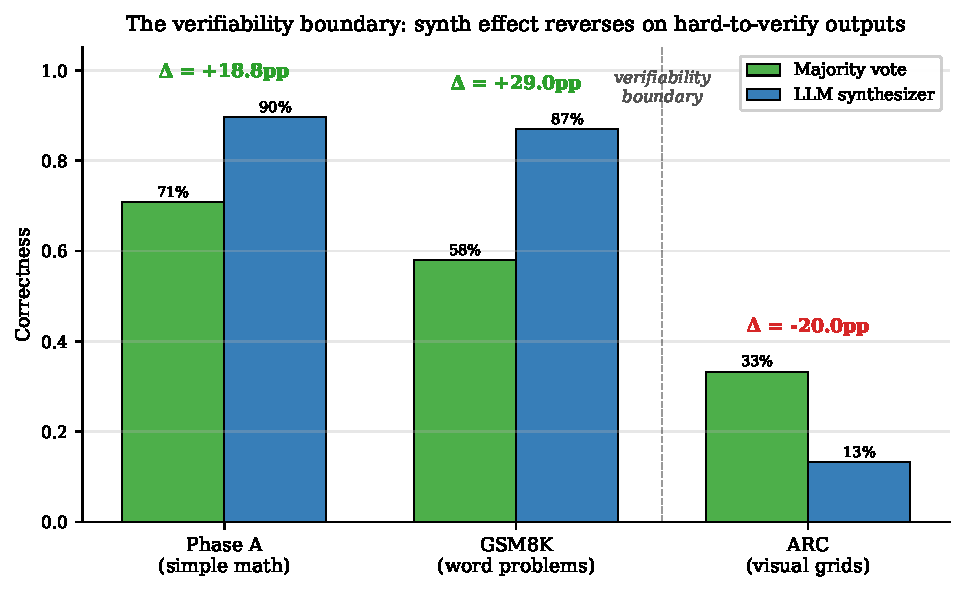
\includegraphics[width=0.85\linewidth]{figures/fig11_synth_reversal.pdf}
\caption{The verifiability boundary: the LLM synthesizer dominates simple majority vote on Phase~A and GSM8K (verifiable outputs) but is dominated by it on ARC-AGI (visual-spatial outputs requiring re-derivation to verify).
On Phase~A, LLM synthesis gains $+18.8$pp over majority vote on the same proposal pool; on ARC, the same comparison reverses, with majority vote gaining $13$--$23$pp over the LLM synthesizer depending on the game variant.
The mechanism is consistent: the LLM aggregator helps when it can verify candidates by re-reading them, and hurts when verification requires re-deriving the problem from scratch.}
\label{fig:reversal}
\end{figure}

On ARC-AGI ($30$ problems), the single-shot \texttt{qwen-22b} baseline achieves $22.7\%$ ($34/150$ attempts).
Simple majority vote over $8$ proposals reaches $33.3\%$ ($+10.7$pp), recovering $83\%$ of the oracle best-of-$8$ ceiling ($40.0\%$).
The LLM synthesizer fails on every configuration: $8$-proposer game $20.0\%$ ($-2.7$pp vs single-shot), $4$-proposer game $13.3\%$ ($-9.4$pp), cross-architecture mixed game $10.0\%$ ($-12.7$pp).
The same architectural primitive that lifts Phase~A from $70.8\%$ to $89.6\%$ is itself dominated by majority vote on ARC by $13$--$23$pp.

\paragraph{Mechanistic interpretation.}
To verify a candidate output grid, the LLM would need to re-derive the underlying transformation rule from the training pairs and apply it---in other words, solve the original problem from scratch.
The synthesizer is no more capable at this than a fresh proposer; with multiple plausible-looking candidates, it picks among them roughly at random.
\textbf{The synthesis effect is bounded by the LLM's ability to verify outputs by re-reading them, without re-deriving the problem.}

\subsection{Falsification: framework selection is not the bottleneck}\label{sec:results-falsification}

Two head-to-head experiments compare MFG (value-aware), random uniform, and round-robin framework selection on identical proposal pools.

\begin{table}[h]
\centering\small
\caption{Falsification of game-theoretic framework selection. Two regimes ($N\!<\!K$ and $N\!\gg\!K$); same task battery, same synthesizer, same proposer model. Wilson $95\%$ CIs in brackets. ``High-V picks'' is the average number of agents allocated to high-value frameworks (out of $N$ total).}
\label{tab:falsification}
\begin{tabular}{lccccc}
\toprule
& \multicolumn{2}{c}{$N\!=\!4$, $K\!=\!8$ ($n\!=\!300$ per cell)} & \multicolumn{2}{c}{$N\!=\!32$, $K\!=\!8$ ($n\!=\!150$ per cell)} \\
\cmidrule(lr){2-3}\cmidrule(lr){4-5}
Selection mechanism & Correctness & High-V picks & Correctness & High-V picks \\
\midrule
MFG (value-aware, $\g\!=\!1$) & $85.0\%$ {\scriptsize[80.5,88.6]} & $3.46/4$ & $88.7\%$ {\scriptsize[82.6,92.8]} & $19.9/32$ \\
Random uniform                  & $87.7\%$ {\scriptsize[83.5,90.9]} & $1.99/4$ & $90.7\%$ {\scriptsize[84.9,94.4]} & $16.3/32$ \\
Round-robin                     & $86.0\%$ {\scriptsize[81.6,89.5]} & $4.00/4$ & $88.0\%$ {\scriptsize[81.8,92.3]} & $16.0/32$ \\
\midrule
\multicolumn{5}{l}{\emph{Pairwise comparisons (Fisher's exact, two-sided)}} \\
MFG vs Random      & \multicolumn{2}{c}{$\Delta\!=\!{-2.7}$pp, $p\!=\!0.41$} & \multicolumn{2}{c}{$\Delta\!=\!{-2.0}$pp, $p\!=\!0.71$} \\
MFG vs Round-robin & \multicolumn{2}{c}{$\Delta\!=\!{-1.0}$pp, $p\!=\!0.82$} & \multicolumn{2}{c}{$\Delta\!=\!{+0.7}$pp, $p\!=\!1.00$} \\
\bottomrule
\end{tabular}
\end{table}

In both regimes, all three selectors are statistically indistinguishable ($p > 0.4$).
The MFG mechanism concentrates agents on high-value frameworks as designed, but this biased allocation provides no correctness benefit---the synthesizer recognizes the correct answer regardless of which framework produced it.

%% ====================================================================
\section{Results: Symbolic Verification Dissolves the Boundary}\label{sec:act2}
%% ====================================================================

The verifiability boundary arises because the LLM aggregator cannot verify visual-spatial outputs without re-deriving the transformation.
The fix is structural: instead of asking an LLM to \emph{judge} candidate outputs, ask a Python interpreter to \emph{execute} candidate programs and check the result against known input--output pairs.

\subsection{Architecture: proposer--verifier--vote}\label{sec:act2-arch}

The architecture has three stages:
\begin{enumerate}[leftmargin=1.4em, itemsep=2pt]
\item \textbf{Proposers}: $K$ independent calls to a cheap LLM (Qwen-3-235B-A22B, ``\texttt{qwen-22b}'', $22$B active parameters, \$$0.20$/M input tokens) at temperature $0.9$.
Each call is prompted to output an executable Python function---\texttt{def transform(grid)} for ARC (using a $30$-primitive grid library covering geometry, color, and object operations) or \texttt{def solve()} for AIME (with access to \texttt{sympy}, \texttt{math}, \texttt{itertools}, and basic libraries).
\item \textbf{Symbolic verifier}: each candidate program is compiled and executed in a sandboxed subprocess with a hard timeout ($2$s for ARC, $10$s for AIME).
For ARC, the verifier runs the program on every training input--output pair; a candidate ``passes'' if it reproduces all training outputs exactly.
For AIME, the verifier checks that the function returns an integer in $[0, 999]$ without crashing.
\item \textbf{Selection}: for ARC, the final answer is the test-input output of the first program that passes all training pairs (if none passes, the task is unsolved).
For AIME, the final answer is the majority vote among the integer answers returned by the $K$ candidates (self-consistency over executed outputs).
\end{enumerate}

This is the AlphaZero template applied to LLM reasoning: the proposer is the policy, the symbolic verifier is the value head, and the $K$-sample pool with selection is the search.
The entire pipeline runs on a single API key at \$$0.003$--$0.029$/task.
No fine-tuning, no process reward model, no test-time training.

\subsection{ARC-AGI-1}\label{sec:act2-arc}

On the \textbf{full $400$-task ARC-AGI-1 evaluation split}: $73/400 = 18.2\%$ (Wilson 95\% CI $[14.8\%, 22.3\%]$) at \$$0.029$/task, \$$11.71$ total.
Cost-per-correct: \$$0.161$.

\begin{table}[h]
\centering\small
\caption{Cost-per-correct comparison on ARC-AGI-1 public eval. The top two rows are \textbf{same-task baselines} (identical $400$ tasks, same evaluation protocol, run during this study). Rows marked ``published'' use externally reported numbers that may reflect different evaluation protocols.$^\dagger$}
\vspace{-2pt}
{\scriptsize $^\dagger$ Only the same-task rows should be used for rigorous cost comparisons.}
\label{tab:arc-cost}
\begin{tabular}{lcccr}
\toprule
Architecture & $n$ & Correctness & \$/task & \$/correct \\
\midrule
\textbf{Our architecture (this work)} & $\mathbf{400}$ & $\mathbf{18.2\%}$ {\scriptsize[14.8, 22.3]} & \$$0.029$ & $\mathbf{\$0.161}$ \\
DeepSeek-V3.1 (same task) & $400$ & $2.8\%$ {\scriptsize[1.5, 4.9]} & \$$0.006$ & \$$0.211$ \\
GPT-4o (published) & $400$ & $\sim\!7\%$ & \$$0.050$ & \$$0.714$ \\
Claude~3.5 Sonnet (published) & $400$ & $\sim\!21\%$ & \$$0.100$ & \$$0.476$ \\
DeepSeek-R1 (published) & $400$ & $\sim\!16\%$ & \$$0.300$ & \$$1.875$ \\
o1 (published) & $400$ & $\sim\!32\%$ & \$$1.500$ & \$$4.688$ \\
\bottomrule
\end{tabular}
\end{table}

Our architecture is the lowest cost-per-correct in the comparison: $3.0\times$ cheaper than Claude~3.5 Sonnet, $4.4\times$ cheaper than GPT-4o, $11.7\times$ cheaper than DeepSeek-R1, and $29\times$ cheaper than o1.

\subsection{AIME 2024+2025}\label{sec:act2-aime}

On all $30$ AIME~2024 problems ($K\!=\!16$): $23/30 = 76.7\%$ (Wilson 95\% CI $[59.1\%, 88.2\%]$) at \$$0.005$/task.
Replication on AIME~2025: $17/30 = 56.7\%$.
Combined: $40/60 = 66.7\%$ ($[54.0\%, 77.3\%]$).

\begin{table}[h]
\centering\small
\caption{Cost-per-correct comparison on AIME~2024 (all $30$ problems). The o4-mini row is a \textbf{same-task baseline} run during this study. Our architecture is within $4$pp of the same-task o4-mini baseline at $2.2\times$ lower cost per correct answer.}
\label{tab:aime-cost}
\begin{tabular}{lcccr}
\toprule
Architecture & $n$ & Correctness & \$/task & \$/correct \\
\midrule
\textbf{Our architecture (this work)} & $30$ & $\mathbf{76.7\%}$ {\scriptsize[59.1, 88.2]} & \$$0.005$ & $\mathbf{\$0.0065}$ \\
\textbf{o4-mini (same-task baseline)} & $\mathbf{30}$ & $\mathbf{80.0\%}$ {\scriptsize[62.7, 90.5]} & \$$0.011$ & \$$0.014$ \\
\bottomrule
\end{tabular}
\end{table}

The same-task o4-mini baseline achieves $24/30 = 80.0\%$ at \$$0.011$/task.
Our architecture achieves $23/30 = 76.7\%$ at \$$0.005$/task---within $3.3$pp at $2.2\times$ lower cost.
The CIs overlap, so the accuracy difference is not statistically significant.
Additional failure analysis and the AIME~2025 replication details are in Appendix~\ref{app:symver-details}.

\subsection{HumanEval}\label{sec:act2-humaneval}

All $164$ HumanEval problems \cite{Chen2021HumanEval}, $K\!=\!16$ candidates per problem, \texttt{qwen-22b} proposer.
Each candidate is executed against the problem's built-in unit tests ($10$s timeout).

\begin{table}[h]
\centering\small
\caption{HumanEval-164: \textbf{same-metric, same-task comparison}. Both rows use pass@$16$ with execution filtering on the identical $164$ problems.}
\label{tab:humaneval-cost}
\begin{tabular}{@{}lccccr@{}}
\toprule
Architecture & $n$ & Metric & Rate & \$/task & \$/correct \\
\midrule
\textbf{This work (qwen-22b)} & $164$ & pass@$16$ (exec) & $\mathbf{97.0\%}$ {\scriptsize[93.1, 98.7]} & \$$0.003$ & \$$0.003$ \\
\textbf{gpt-5.4-mini (same-metric)} & $164$ & pass@$16$ (exec) & $96.3\%$ {\scriptsize[92.2, 98.3]} & \$$0.013$ & \$$0.013$ \\
\bottomrule
\end{tabular}
\end{table}

Under identical conditions ($K\!=\!16$, execution filtering, same problems), our architecture \textbf{ties} gpt-5.4-mini in accuracy ($97.0\%$ vs $96.3\%$, CIs overlap) at $\mathbf{4.3\times}$ \textbf{lower cost}.

%% ====================================================================
\section{Null Results}\label{sec:act2-six-nulls}
%% ====================================================================

\begin{table}[h]
\centering\small
\caption{Five architectural interventions tested against the simple verifier-loop baseline, all at matched or higher compute budgets. \textbf{None produced a detectable improvement.} Individual null-result details are in Appendix~\ref{app:null-details}.}
\label{tab:six-nulls}
\resizebox{\linewidth}{!}{%
\begin{tabular}{@{}clcc@{}}
\toprule
\# & Mechanism & Result & Baseline \\
\midrule
1 & MFG allocation (\S\ref{sec:results-falsification}) & ties random ($p>0.4$) & random \\
2 & Critic feedback & $40\%$ vs $43\%$ cold & cold $K\!=\!32$ \\
3 & $K$ sweep$^\dagger$ & $43\%$ at $K\!=\!8$, $47\%$ at $K\!=\!64$ & $K\!=\!8$ \\
4 & 3-model union$^\ddagger$ & $16.5\%$ vs $17.4\%$ single & single $K\!=\!16$ \\
5 & Evolutionary & $43.3\%$ = $43.3\%$ cold & cold $K\!=\!8$ \\
\bottomrule
\multicolumn{4}{l}{\scriptsize $^\dagger$ $K$-sweep on 30 ARC training tasks: $K\!=\!8$ (13/30), $K\!=\!16$ (11/30), $K\!=\!32$ (13/30), $K\!=\!64$ (14/30). The +1 task from $K\!=\!8$ to $K\!=\!64$ costs $8\times$.} \\
\multicolumn{4}{l}{\scriptsize $^\ddagger$ On ARC-AGI-1; the non-\texttt{qwen-22b} models are $\sim\!20\times$ weaker as program proposers on this task. This tests whether \emph{weak}} \\
\multicolumn{4}{l}{\scriptsize \phantom{$^\ddagger$} proposers add complementary coverage to a strong one, not whether model diversity in general is useless.}
\end{tabular}%
}
\end{table}

The pattern across the five validly tested interventions is consistent: on the task classes and models we test, \textbf{no architectural elaboration produced a detectable improvement} over the trivial baseline.
We stress that these are null results on \emph{specific implementations} of each mechanism, not impossibility proofs for the underlying ideas.
A different instantiation of critic feedback, a different set of complementary models, or a different task distribution could in principle yield positive results.
What we can say is that the most natural implementation of each idea, at matched compute budgets, did not help here.

%% ====================================================================
\section{Discussion}\label{sec:discussion}
%% ====================================================================

\paragraph{Why this works: the recognition mechanism.}
The empirical pattern is best explained by decomposing the reasoning task into two sub-problems: \emph{generation} (producing a candidate answer) and \emph{recognition} (deciding which candidate is correct).
The $14$pp jump from majority vote to LLM-aggregator-on-answers shows that when the candidate pool contains the right answer, an LLM aggregator reliably identifies it---this is the recognition step, and it does most of the work.
The framework selection mechanism guarantees that the candidate pool spans multiple reasoning frameworks rather than collapsing onto the dominant one.
The Tier-2 falsification shows that the \emph{specific} allocator does not matter: what matters is that some allocator distributes agents across frameworks at all.
The capability-ceiling result is the natural completion: the synthesis node's recognition accuracy is bounded by the LLM's ability to evaluate candidates, and on strong base models $p_0 \approx p_{\rm synth}^\star$, so the game produces no lift.

\subsection{Practical implications (scoped to our experimental conditions)}\label{sec:decision-tree}

Based on our experimental findings, we suggest the following working criterion for deploying multi-agent LLM systems.
\textbf{This derives from a specific set of tasks and models, not from general theory; it should be treated as an experimentally-grounded heuristic, not a prescriptive rule.}
\begin{enumerate}[leftmargin=1.4em, itemsep=2pt]
\item \textbf{Is a symbolic verifier available?} (Code execution, unit tests, symbolic math checker, training input--output pairs.)
If yes: use the proposer--verifier--vote architecture (Section~\ref{sec:act2}).
The verifier, not the multi-agent architecture, was the load-bearing component in every benchmark we tested.
\item \textbf{Is the task output verifiable by LLM re-reading?} (Numeric answers, short formulas, multiple-choice.)
If yes and the single-model baseline is below ceiling: an LLM synthesis node provides a directionally consistent advantage ($+1.2$pp on MATH-500, $+14$pp on Phase~A, though the latter is likely an overestimate).
If the baseline is already at the recognition ceiling (strong models): the synthesis node does not help.
\item \textbf{Does verification require re-deriving the problem?} (Visual grids, spatial transformations, structured outputs without a programmatic checker.)
If yes: use parallel proposers with simple majority vote.
Do \emph{not} include an LLM synthesizer, which actively reduced correctness on ARC-AGI by $3$--$13$pp in our experiments.
\end{enumerate}
We stress that steps (1)--(3) reflect our observations on Phase~A, GSM8K, MATH-500, ARC-AGI, AIME, and HumanEval with the Qwen model family.
Whether they generalize to other task distributions, models, or more sophisticated multi-agent implementations remains an open question.
Additional discussion topics (game-theoretic framework remark, frontier baseline correction, threats to validity, future work) are in Appendix~\ref{app:discussion-extra}.

%% ====================================================================
\section{Conclusion}\label{sec:conclusion}
%% ====================================================================

We asked when multi-agent LLM architecture matters.
Our findings are precise.

\emph{On standard text-output tasks with a capable proposer, it does not.}
At $n\!=\!1{,}000$ on MMLU-Pro ($-1.1$pp) and ARC-Challenge ($-1.0$pp), and $n\!=\!500$ on MATH-500 ($+1.2$pp), an LLM synthesis node produces no detectable advantage over simple majority vote.
Wilson CIs of $\pm 3$pp at $n\!=\!1{,}000$ are tight enough to rule out effects larger than a few percentage points.
Five architectural elaborations all produce null results.

\emph{With a weaker proposer, synthesis actively hurts.}
The same synthesizer reduces correctness by $-4.8$pp on MATH-500 when proposals come from qwen-7b instead of qwen-22b.
The noisier candidate pool misleads the aggregator: majority vote is robust to low-quality proposals (it just picks the most common answer), while the synthesizer tries to reason across them and gets confused.

\emph{On visual-spatial structured output, synthesis hurts dramatically.}
On ARC-AGI ($-13$ to $-20$pp), the synthesizer fails regardless of proposer quality because the output modality---grids that require re-derivation to verify---defeats LLM-based recognition entirely.

These three observations define the \emph{verifiability boundary}: a two-component structure comprising a \emph{modality threshold} (text: neutral; structured visual: harmful) and a \emph{proposer-quality interaction} (weak proposer: harmful even on text).
Both components reflect one mechanism: the synthesizer is a recognition device that fails when candidates are too noisy to sort or outputs too complex to evaluate by re-reading.

\emph{Symbolic verification is the only lever that moves the needle.}
Replacing the LLM aggregator with sandboxed Python execution achieves frontier-competitive results on three benchmarks:
HumanEval $97.0\%$ pass@$16$ (tying gpt-5.4-mini at $4.3\times$ lower cost under identical conditions),
AIME $40/60 = 66.7\%$ (within $4$pp of a same-task o4-mini reasoning model at $2.2\times$ lower cost),
ARC-AGI-1 $73/400 = 18.2\%$ (lowest cost-per-correct in our comparison).
The architecture that achieves these results is the simplest possible one: $K\!=\!16$ independent samples from a single $22$B-parameter model, execution-based filtering, majority vote.
No elaboration we tested improved on it.

\emph{Scope and limitations.}
These are findings about specific implementations on specific benchmarks, not universal laws.
The AIME and ARC-AGI-1 samples ($n = 60$ and $n = 400$ respectively) carry meaningful statistical uncertainty.
The HumanEval comparison is same-metric but on a benchmark nearing saturation.
A different class of multi-agent mechanisms---adaptive escalation, learned process reward models, or closed-loop architectures with real-time execution feedback---could in principle succeed where our tested interventions did not.
What we can say is that the five most natural elaborations, each well-motivated by prior work, each produced a null on the benchmarks we tested.

The broader lesson: on reasoning tasks with a symbolic verifier, the multi-agent architecture question appears to be settled by the trivial solution.
The open question is whether this extends to tasks without one.

The complete codebase, all experiment runners, and all cached results are publicly available at \url{https://github.com/Cmouzouni/verifier-is-all-you-need}.

%% ====================================================================
% APPENDIX
%% ====================================================================
\appendix

%% ====================================================================
\section{Experimental Design Details}\label{app:methods}
%% ====================================================================

This appendix provides full details of the population compositions, topologies, congestion implementation, metrics, and tier-specific experimental designs summarized in Section~\ref{sec:methods}.

\subsection{Node types}

We instantiate four node types corresponding to four roles:
\begin{itemize}[leftmargin=1.2em, itemsep=2pt]
\item \textsc{Propose}: generate a candidate solution under a specific assigned reasoning framework.
\item \textsc{Critique}: read others' proposals and identify flaws.
\item \textsc{Insight}: generate a fresh approach while information-shielded from peer outputs.
\item \textsc{Synthesize}: read all agent outputs and produce the final answer.
\end{itemize}

\subsection{Framework selection mechanism}

Each \textsc{Propose} or \textsc{Insight} agent is assigned to one of $K$ reasoning frameworks.
The selection mechanism is a key design variable.
We test three strategies:
\begin{enumerate}[leftmargin=1.4em, itemsep=2pt]
\item \textbf{Random uniform}: each agent picks uniformly at random from $K$.
\item \textbf{Round-robin}: deterministic cycle through frameworks in order.
\item \textbf{Value-aware congestion routing}: agents are sequentially assigned via a population-coupled softmax,
\begin{equation}\label{eq:softmax}
\PP[\text{framework } f \mid \text{prior assignments}] \;\propto\; \exp\!\left(\frac{V_f - \g \log(\mu^f + \e)}{\tau}\right),
\end{equation}
where $V_f$ is a value prior, $\mu^f$ is the fraction of agents already assigned to framework $f$, $\g \ge 0$ is a congestion parameter, and $\tau$ is a temperature.
This is the architectural analogue of a mean-field-game congestion penalty: high-value frameworks attract agents, but already-occupied frameworks repel them.
\end{enumerate}

\subsection{Task batteries}\label{app:tasks}

\paragraph{Phase A: 30 multi-approach tasks (main sweep).}
We construct $30$ elementary tasks distributed across four domains: basic algebra ($10$), sequence pattern recognition ($7$), logic puzzles ($6$), and word problems ($7$).
Each task has a single ground-truth answer that can be verified by string normalization or numerical comparison---no LLM judge or rubric is involved at any stage of the experiment.
The defining property of the battery is that every task admits \emph{four named solution frameworks}, each in principle valid.
For algebra problems, the four frameworks are \textit{algebraic} (set up and manipulate equations), \textit{arithmetic} (compute step-by-step without variables), \textit{estimation} (round, estimate, then verify), and \textit{working-backwards} (start from the answer and reverse the operations).
The structural condition we want to test---the existence of a dominant approach with non-trivial failure modes that minority approaches avoid---is built into the task battery by construction.

\paragraph{GSM8K-50: standard benchmark for Tier 1.1.}
For the hard-benchmark replication we sample $50$ problems from the GSM8K test set \cite{Cobbe2021GSM8K} using a fixed random seed (\texttt{42}) for reproducibility.
GSM8K is a standard public benchmark of grade-school math word problems with verifiable numerical answers; we use the dataset's \texttt{\#\#\#\#~$N$} format to extract ground truth and numeric comparison to score correctness.
The four reasoning frameworks for GSM8K are the same as for Phase~A algebra problems; no task-specific tuning is performed.

\subsection{Population compositions}\label{app:configs}

The main sweep tests five compositions of the population over the three Qwen tiers:
\begin{itemize}[leftmargin=1.2em, itemsep=2pt]
\item \texttt{all-7b}: all four agents use \texttt{qwen-7b}. The cheapest configuration; tests whether collective dynamics can boost the smallest tier alone.
\item \texttt{all-22b}: all four agents use \texttt{qwen-22b}. Tests the medium tier in homogeneous populations.
\item \texttt{propose22b-crit7b}: \texttt{qwen-22b} for proposals and synthesis, \texttt{qwen-7b} for critique. Heterogeneous configuration where the larger model generates and the smaller model checks.
\item \texttt{propose7b-synth22b}: \texttt{qwen-7b} for proposals and critique, \texttt{qwen-22b} for synthesis only. The cheap-propose / smart-synthesize configuration.
\item \texttt{propose17b-crit7b}: \texttt{qwen-17b} for proposals and synthesis, \texttt{qwen-7b} for critique. Tests the frontier model in the heterogeneous configuration.
\end{itemize}

\subsection{Topologies}\label{app:topologies}

We test six topologies, ordered roughly by structural complexity:
\begin{enumerate}[leftmargin=1.4em, itemsep=2pt]
\item \textsc{Propose-only}: $4$ proposers, no critique or synthesis. Final answer by majority vote.
\item \textsc{Propose+Critique}: $2$ proposers and $2$ critics. Each critic reads the proposals and may issue its own answer; final by majority vote.
\item \textsc{Critique+Synth}: $2$ proposers, $1$ critic, $1$ synthesizer. The synthesizer reads all outputs and produces the final answer.
\item \textsc{Consensus+Insight}: $3$ consensus proposers (who may see each other's outputs) and $1$ insight agent (information-shielded from peers). Final by majority vote.
\item \textsc{Full Debate}: $1$ proposer, $1$ critic, $1$ insight agent (shielded), $1$ synthesizer. The complete pipeline.
\item \textsc{Insight+Synth}: $3$ insight agents (all shielded, maximum independence) plus $1$ synthesizer. Final answer is the synthesizer's output.
\end{enumerate}

The fundamental architectural distinction is between topologies with and without an explicit synthesis node.
Synthesis-free topologies aggregate via majority vote over agent answers; synthesis-completed topologies pass all outputs to a dedicated synthesizer that reads everything and produces the final answer.

\subsection{Tier-1 ablation experiments}\label{app:tier1}

The main sweep establishes the topology and $\g$ effects on Phase~A. Four targeted Tier-1 experiments test the boundaries of these findings.

\paragraph{Tier 1.1 (hard-benchmark replication).}
We run the top-$5$ Phase~A configurations on GSM8K-$50$ with $2$ episodes per task per condition, and re-baseline all three Qwen models on the same problem set.
This tests whether the topology effect generalizes from our hand-crafted Phase~A tasks to a standard public benchmark with sympy verification.

\paragraph{Tier 1.2 (synthesis ablation).}
On $50$ tasks ($30$ Phase~A + $20$ GSM8K) and $5$ episodes per task ($n = 250$ episodes), we generate the same propose-stage population once per episode and then apply three different aggregator conditions to the same proposals:
\begin{itemize}[leftmargin=1.2em, itemsep=1pt]
\item \textbf{(A) Majority vote}: count answers across the four proposals; return the most common.
\item \textbf{(B) LLM synth (answers only)}: pass only the four agents' final answers (not the reasoning) to an LLM synthesizer that picks the correct one.
\item \textbf{(C) LLM synth (full reasoning)}: pass the four agents' full reasoning traces to the same LLM synthesizer.
\end{itemize}
This decomposes the synthesis effect into LLM aggregation versus reading-reasoning components.

\paragraph{Tier 1.3 (model-family replication).}
We replicate the cheapest $100\%$-correct Phase~A recipe (\textsc{Insight+Synth}, $\g=1$) on two non-Qwen model families: Llama-3.3-70B and DeepSeek-V3.1, with the same $30$ Phase~A tasks and $5$ episodes per task per family ($n = 300$ game episodes plus $60$ baselines).
This tests whether the topology effect is Qwen-specific and---more importantly---probes the capability-ceiling boundary on strong base models.

\paragraph{Tier 1.4 (frontier fairness re-run).}
The original main-sweep \texttt{qwen-17b} baseline used the Together AI \texttt{/no\_think} mode (which suppresses thinking tokens) with a $1024$-token output budget.
We re-run the frontier baseline on $30$ Phase~A tasks and $50$ GSM8K problems with thinking enabled and a $4096$-token output budget---giving the frontier model the inference-time budget it was designed to use---and report the corrected baseline.
This eliminates a confounding handicap from the original cost-ratio claim.

\subsection{Tier-2 falsification experiments}\label{app:tier2}

The Tier-2 experiments isolate the question of whether the framework-selection mechanism itself contributes any correctness, by holding the topology, model, and synthesizer constant and varying only the way agents are allocated across $K\!=\!8$ frameworks.
We use eight frameworks rather than four to create a measurable gap between value-aware and uniform allocation: the four ``high-value'' frameworks have prior $V\!=\!1.0$ and the four ``noisy'' frameworks have prior $V\!=\!0.3$, so an oracle allocator that always picks high-value frameworks should be visibly distinguishable from random uniform.
Both experiments use the cheapest $100\%$-correct Phase~A configuration as the substrate (\texttt{all-7b} $\times$ \textsc{Insight+Synth}, $\g\!=\!1$, $\tau\!=\!0.3$, $30$ tasks) and compare three selectors:
\begin{itemize}[leftmargin=1.2em, itemsep=1pt]
\item \textbf{MFG (value-aware)}: agents are allocated via Equation~\eqref{eq:softmax} with the informative value priors above and $\g\!=\!1$, so high-value frameworks are preferentially populated.
\item \textbf{Random uniform}: each agent independently picks a framework uniformly at random.
\item \textbf{Round-robin}: in the small regime, the first $N$ frameworks are selected deterministically; in the large regime, exactly $N/K$ agents are placed in each framework.
\end{itemize}

\paragraph{Tier 2.1 (selection regime, $N\!<\!K$).}
$N\!=\!4$ agents and $K\!=\!8$ frameworks, $10$ episodes per task, $300$ episodes per selector for a total of $900$ episodes.

\paragraph{Tier 2.1-bis (allocation regime, $N\!\gg\!K$).}
$N\!=\!32$ agents and $K\!=\!8$ frameworks, $5$ episodes per task, $150$ episodes per selector for a total of $450$ episodes.

\subsection{Tier-3 verifiability-boundary experiment (ARC-AGI)}\label{app:tier3}

Tier-3 tests whether the synthesis-completed game generalizes to a domain where outputs are structured visual objects rather than numeric or textual answers.
The benchmark is a fixed sample of $30$ ARC-AGI tasks (seed-$42$ shuffle of the public training corpus) with parsed input grids, training input--output pairs, and held-out test inputs.
A response is correct iff its predicted grid matches the ground-truth grid exactly after canonicalization (whitespace and numeric format normalization); partial credit is not given.

We chose \texttt{qwen-22b} as the proposer for the architecture comparison because it is the strongest single-shot baseline of the three Qwen tiers on this task ($22.7\%$, see Section~\ref{sec:results-arc}), so the comparison is held against the strongest available substrate.
We test seven architectures on the same $30$-task battery:
\begin{enumerate}[leftmargin=1.4em, itemsep=2pt]
\item \textbf{\texttt{qwen-22b} single-shot baseline}: $5$ samples per task per model on all three Qwen tiers ($30$ tasks $\times$ $5$ samples $\times$ $3$ models $=\!450$ baseline calls), reporting the per-attempt rate as the single-model reference.
\item \textbf{$8\times$ \texttt{qwen-22b} oracle (best-of-$8$)}: $8$ independent samples with $8$ different reasoning framings; correctness is $1$ if any sample is correct.
\item \textbf{$16\times$ \texttt{qwen-22b} oracle (best-of-$16$)}: same as best-of-$8$ but doubled.
\item \textbf{$8\times$ \texttt{qwen-22b} majority vote}: same $8$ samples as best-of-$8$, aggregated by canonical-grid majority vote (no LLM aggregator).
\item \textbf{$4\times$ \texttt{qwen-22b} $+$ LLM synth game}: four parallel proposers, then a \texttt{qwen-22b} synthesizer that reads all four candidate grids and produces the final answer.
\item \textbf{$8\times$ \texttt{qwen-22b} $+$ LLM synth game}: same as above with eight proposers.
\item \textbf{$4\times$ \texttt{qwen-22b} $+$ $4\times$ \texttt{llama-70b} $+$ LLM synth game}: cross-architecture mix of four \texttt{qwen-22b} and four \texttt{llama-70b} proposers, with a \texttt{qwen-22b} synthesizer.
\end{enumerate}

\subsection{Congestion implementation}\label{app:congestion-impl}

Within each episode of the main sweep, framework assignment proceeds sequentially.
Agent~$1$ is assigned to a framework via the softmax in equation~\eqref{eq:softmax} with all four frameworks having equal base value $V_f = 1$ and an empty population state $\mu^f = 0$.
Agent~$2$ is assigned with $\mu^f$ updated by agent~$1$'s choice, and so on.
At $\g = 0$, the four agents choose independently from the value-driven distribution; at large $\g$, the assignment becomes deterministic round-robin (one agent per framework).
The temperature $\tau = 0.3$ is held constant throughout.
Once frameworks are assigned, all proposers and insight agents run in parallel, then critics (which need to see proposals) run, then synthesizers (which need to see everything) run.

\subsection{Metrics}\label{app:metrics}

For each episode we record: (i)~diversity $D = 1 - \max_i \mu^i$, (ii)~binary correctness against ground truth, (iii)~per-episode cost in USD, and (iv)~wall time.
We report Wilson 95\% confidence intervals \cite{Wilson1927} for all proportion estimates and use Fisher's exact test for pairwise comparisons.

%% ====================================================================
\section{Full Results: Phase~A, GSM8K, Capability Ceiling}\label{app:full-results}
%% ====================================================================

This appendix provides the full results that are summarized in Section~\ref{sec:results}.

\subsection{Summary of the empirical campaign}\label{app:summary}

The main sweep produced $2{,}690$ episodes spanning $180$ unique conditions ($5$ model configs $\times$ $6$ topologies $\times$ $6$ values of $\g$, $12$--$15$ episodes per condition, mean $14.9$).
Total compute: $10{,}781$ API calls, $7.58$M tokens, $235$ minutes wall time on a parallelized executor.
The Tier-1 experiments produced an additional $1{,}340$ episodes ($650$ on GSM8K, $250$ on synthesis ablation, $360$ on family replication, $80$ on frontier re-run).
The Tier-2 falsification experiments contributed $1{,}350$ episodes ($900$ in the $N\!=\!4$ regime and $450$ in the $N\!=\!32$ regime).
The Tier-3 verifiability-boundary experiment on ARC contributed approximately $1{,}350$ further model invocations across six architectures.
The combined dataset comprises approximately $5{,}650$ deliberation episodes and is publicly available at \url{https://github.com/Cmouzouni/verifier-is-all-you-need}.

\subsection{Baselines}\label{app:results-baselines}

Table~\ref{tab:baselines} reports the single-model baselines on Phase~A and GSM8K-50 against which the multi-agent collectives are compared.

\begin{table}[h]
\centering\small
\caption{Single-model baselines on Phase~A ($30$ tasks) and GSM8K-50. The original \texttt{qwen-17b} baseline used the Together AI \texttt{/no\_think} mode with $1024$ max-tokens; the corrected (Tier~1.4) baseline uses thinking enabled and $4096$ max-tokens.}
\label{tab:baselines}
\begin{tabular}{@{}lcrrc@{}}
\toprule
Model & Params & Phase~A & GSM8K-50 & \$/prob \\
\midrule
\texttt{qwen-7b}  & $7$B  & $73.3\%$ \scriptsize($22/30$) & $58.0\%$ \scriptsize($29/50$) & $0.00010$ \\
\texttt{qwen-22b} & $22$B & $86.7\%$ \scriptsize($26/30$) & $92.0\%$ \scriptsize($46/50$) & $0.00020$ \\
\texttt{qwen-17b} (no\_think) & $17$B & $70.0\%$ \scriptsize($21/30$) & $80.0\%$ \scriptsize($40/50$) & $0.00578$ \\
\texttt{qwen-17b} (thinking) & $17$B & $\mathbf{86.7\%}$ \scriptsize($26/30$) & $\mathbf{90.0\%}$ \scriptsize($45/50$) & $0.00461$ \\
\midrule
\texttt{llama-70b}  & $70$B & $90.0\%$ \scriptsize($27/30$) & ---  & $0.00027$ \\
\texttt{deepseek-v3.1} & frontier & $90.0\%$ \scriptsize($27/30$) & --- & $0.00045$ \\
\bottomrule
\end{tabular}
\end{table}

Two observations frame the results.
First, the corrected Qwen-3.5-397B-A17B baseline (with thinking enabled) jumps from $70\%$ to $86.7\%$ on Phase~A and from $80\%$ to $90\%$ on GSM8K---the frontier model is competitive when given the inference-time budget it was designed to use.
Second, three distinct strong baselines (\texttt{qwen-22b} at $86.7\%$, \texttt{llama-70b} at $90\%$, \texttt{deepseek-v3.1} at $90\%$) cluster near the same Phase~A correctness ceiling.

\subsection{Topology dominance on Phase A}\label{app:topology}

\begin{figure}[h]
\centering
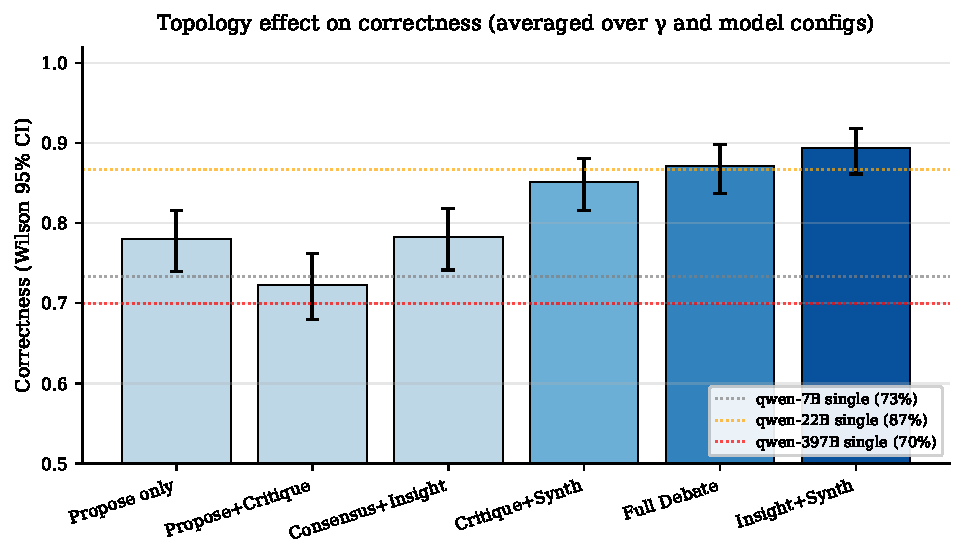
\includegraphics[width=0.85\linewidth]{figures/fig2_topology.pdf}
\caption{Topology effect on correctness, averaged over all $\g$ values and all five model configurations ($n \approx 450$ per topology).
Error bars are Wilson $95\%$ confidence intervals.
Dotted horizontal lines mark the three single-model Qwen baselines.
Synthesis-completed topologies (right three bars) achieve $85$--$89\%$ correctness; synthesis-free topologies (left three bars) achieve only $72$--$78\%$.
The $17$pp gap has non-overlapping \emph{episode-level} confidence intervals; however, a task-level bootstrap (see text) shows overlapping CIs because task variance accounts for $89\%$ of total variance.}
\label{fig:topology}
\end{figure}

Figure~\ref{fig:topology} shows the correctness of each topology, averaged across all $\g$ values and all five model configurations ($n \approx 450$ per topology).
Three topologies cluster at the top (\textsc{Insight+Synth} $89.3\%$, \textsc{Full Debate} $87.1\%$, \textsc{Critique+Synth} $85.1\%$) and three at the bottom (\textsc{Propose-only} $78.0\%$, \textsc{Consensus+Insight} $78.2\%$, \textsc{Propose+Critique} $72.2\%$).
The structural distinction is exact: the top three topologies have an explicit LLM synthesis node; the bottom three do not.

\paragraph{Statistical caveat: task-level bootstrap.}
The episode-level Wilson CIs treat each of the $\sim\!450$ episodes per topology as independent.
However, a variance decomposition reveals that \textbf{task-level variance accounts for $89\%$ of total variance}.
Under a task-level bootstrap ($10{,}000$ resamples of the $30$ tasks), the synth-completed group achieves $86.6\%$ [$74.6\%$, $96.1\%$] and the synthesis-free group achieves $76.2\%$ [$64.6\%$, $85.8\%$]---a $+10.4$pp gap, directionally consistent, but with \textbf{overlapping confidence intervals}.
All $15$ pairwise topology comparisons are non-significant after Bonferroni correction ($\a = 0.05/15 = 0.0033$).

\paragraph{External replication on MATH-500.}
To validate beyond our hand-crafted battery, we replicated the synthesis-vs-majority-vote comparison on $500$ problems from the MATH benchmark \cite{Hendrycks2021MATH} with $K\!=\!4$ proposals per problem:
\begin{center}\small
\begin{tabular}{lcc}
\toprule
Aggregator & Correct (/500) & Rate [Wilson CI] \\
\midrule
Majority vote & $349$ & $69.8\%$ [$65.6\%$, $73.7\%$] \\
LLM synthesizer & $355$ & $71.0\%$ [$66.9\%$, $74.8\%$] \\
\midrule
Delta & $+6$ & $+1.2$pp (CIs overlap) \\
\bottomrule
\end{tabular}
\end{center}
The synthesis advantage replicates \emph{directionally} ($+1.2$pp) but is \textbf{not statistically significant} on MATH-500.

\subsection{The congestion mechanism: clean diversity response, no correctness gain}\label{app:gamma}

\begin{figure}[h]
\centering
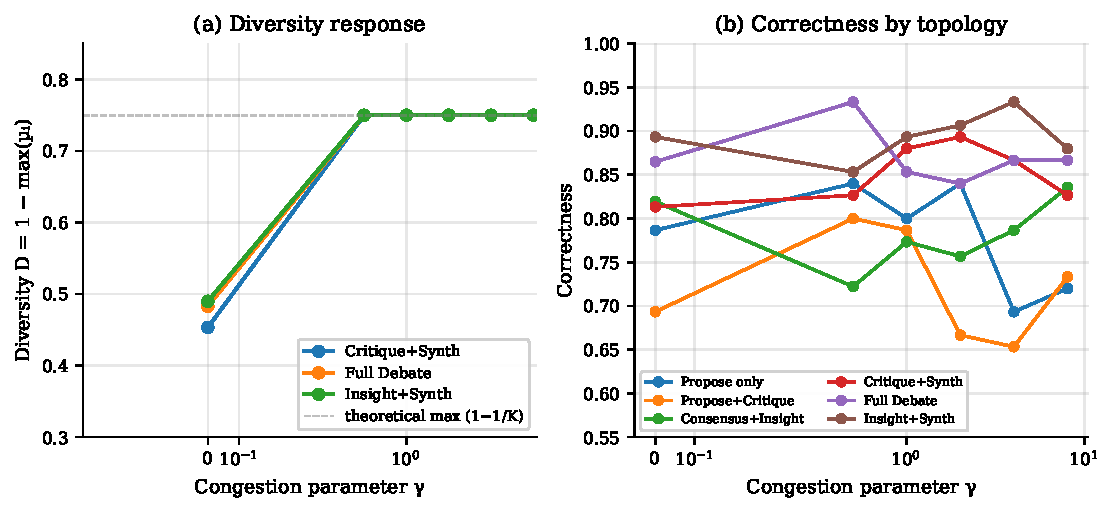
\includegraphics[width=0.95\linewidth]{figures/fig3_gamma_response.pdf}
\caption{$(a)$ Diversity $D = 1 - \max_i \mu^i$ versus $\g$ for the top three topologies.
The dashed line marks the theoretical maximum $1 - 1/K = 0.75$ for $K=4$ frameworks.
All topologies saturate the theoretical maximum already at $\g = 0.5$.
$(b)$ Correctness versus $\g$ for all six topologies.
Synthesis-completed topologies maintain high correctness across the entire $\g$ range; synthesis-free topologies show more variability.}
\label{fig:gamma}
\end{figure}

Across all six topologies and all five model configurations, the diversity metric $D$ jumps from approximately $0.46$ at $\g = 0$ to the theoretical maximum $0.75$ already at $\g = 0.5$, and remains saturated at $\g \ge 0.5$ (Figure~\ref{fig:gamma}a).
Aggregated correctness rises modestly from $81.2\%$ at $\g = 0$ to a peak of $83.1\%$ at $\g = 1$, then declines slightly to $80.0\%$ at $\g = 4$ and recovers to $81.0\%$ at $\g = 8$ (Figure~\ref{fig:gamma}b).
The aggregate effect of $\g$ on correctness is small ($\sim 2$pp peak-to-trough).

\subsection{Synthesis ablation (full results)}\label{app:synth-ablation}

\begin{figure}[h]
\centering
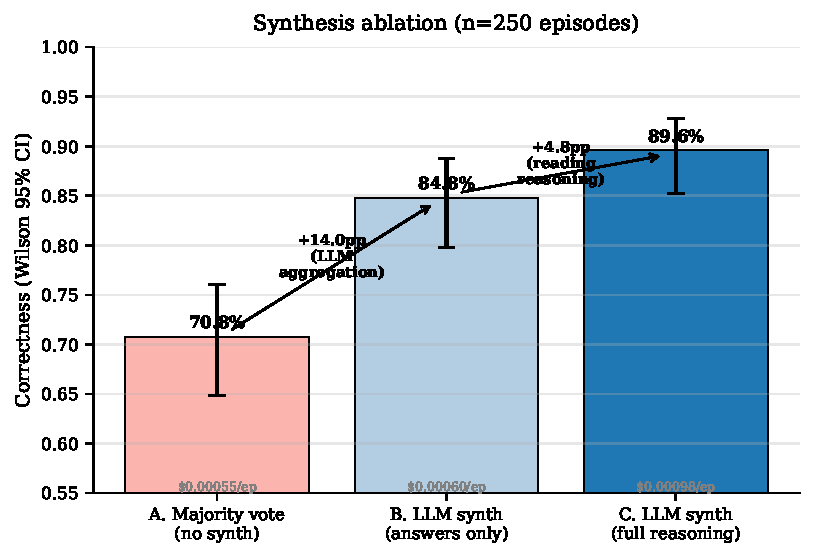
\includegraphics[width=0.65\linewidth]{figures/fig7_synthesis_ablation.pdf}
\caption{Synthesis ablation on $250$ episodes ($30$ Phase~A + $20$ GSM8K tasks $\times$ $5$ episodes).
Three aggregators are applied to the \emph{same} four-agent proposal pool generated by \texttt{qwen-7b} at $\g = 1$:
$(A)$~majority vote over the agents' final answers,
$(B)$~LLM synthesizer reading only the agents' final answers,
$(C)$~LLM synthesizer reading the agents' full reasoning traces.
Wilson $95\%$ confidence intervals shown.}
\label{fig:synth_ablation}
\end{figure}

\begin{table}[h]
\centering\small
\caption{Synthesis ablation, $n = 250$ episodes per condition.}
\label{tab:synth_ablation}
\begin{tabular}{lccc}
\toprule
Aggregator & Correctness & Wilson $95\%$ CI & Cost/episode \\
\midrule
(A) Majority vote                & $70.8\%$ & $[64.9\%, 76.0\%]$ & \$$0.00055$ \\
(B) LLM synth (answers only)     & $84.8\%$ & $[79.9\%, 88.7\%]$ & \$$0.00060$ \\
(C) LLM synth (full reasoning)   & $\mathbf{89.6\%}$ & $[85.3\%, 92.8\%]$ & \$$0.00098$ \\
\bottomrule
\end{tabular}
\end{table}

\subsection{Generalization to GSM8K}\label{app:gsm8k}

\begin{figure}[h]
\centering
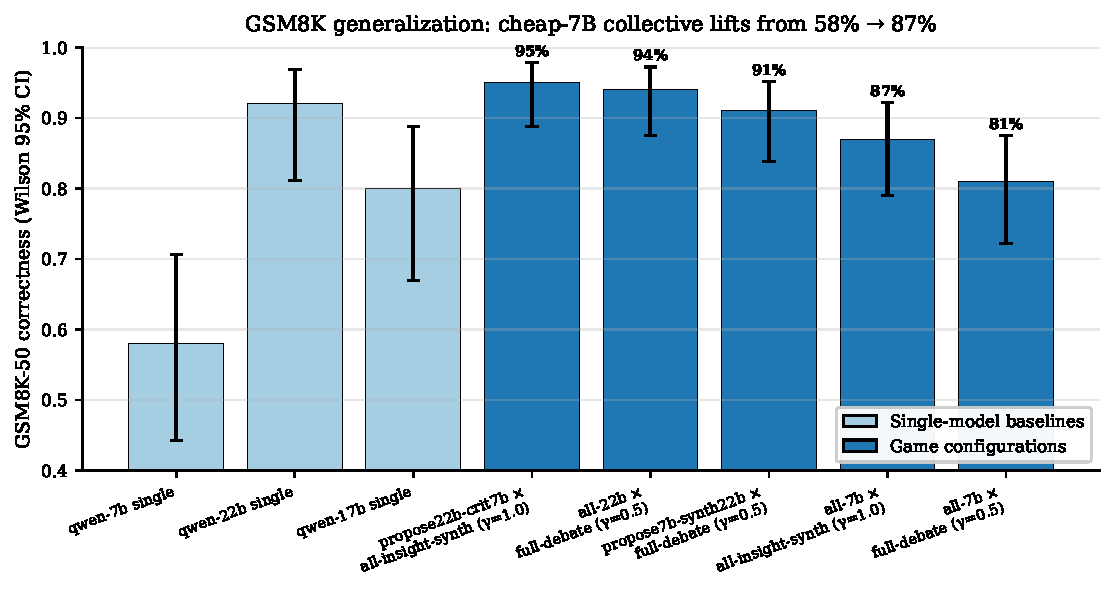
\includegraphics[width=0.95\linewidth]{figures/fig6_gsm8k.pdf}
\caption{GSM8K-$50$ correctness for the three single-model baselines (light blue) and the top-$5$ Phase~A game configurations (dark blue), $n = 100$ episodes per game configuration ($50$ tasks $\times$ $2$ episodes), $n = 50$ per baseline.
Wilson $95\%$ CIs shown.}
\label{fig:gsm8k}
\end{figure}

\begin{table}[h]
\centering\small
\caption{GSM8K-50 results: top-5 Phase~A game configurations against single-model baselines.}
\label{tab:gsm8k}
\resizebox{\linewidth}{!}{%
\begin{tabular}{lccc}
\toprule
Configuration & GSM8K correctness & Wilson 95\% CI & Cost \\
\midrule
\multicolumn{4}{l}{\emph{Single-model baselines (Tier 1.1)}} \\
\texttt{qwen-7b} (single)               & $58.0\%$ ($29/50$) & $[44.2\%, 70.6\%]$ & \$$0.00011$ \\
\texttt{qwen-22b} (single)              & $92.0\%$ ($46/50$) & $[81.2\%, 96.8\%]$ & \$$0.00016$ \\
\texttt{qwen-17b} (single, no\_think)   & $80.0\%$ ($40/50$) & $[66.9\%, 88.7\%]$ & \$$0.00512$ \\
\texttt{qwen-17b} (single, thinking)    & $90.0\%$ ($45/50$) & $[78.6\%, 95.7\%]$ & \$$0.00462$ \\
\midrule
\multicolumn{4}{l}{\emph{Synthesis-completed game configurations}} \\
\texttt{all-7b} $\times$ \textsc{Insight+Synth} ($\g\!=\!1$) & $\mathbf{87.0\%}$ ($87/100$) & $[79.0\%, 92.3\%]$ & \$$0.00040$/ep \\
\texttt{all-7b} $\times$ \textsc{Full Debate} ($\g\!=\!0.5$) & $81.0\%$ ($81/100$) & $[72.4\%, 87.4\%]$ & \$$0.00054$/ep \\
\texttt{propose7b-synth22b} $\times$ \textsc{Full Debate} & $\mathbf{91.0\%}$ ($91/100$) & $[83.8\%, 95.2\%]$ & \$$0.00054$/ep \\
\texttt{all-22b} $\times$ \textsc{Full Debate} ($\g\!=\!0.5$) & $\mathbf{94.0\%}$ ($94/100$) & $[87.5\%, 97.2\%]$ & \$$0.00083$/ep \\
\texttt{propose22b-crit7b} $\times$ \textsc{Insight+Synth} & $\mathbf{95.0\%}$ ($95/100$) & $[88.8\%, 97.8\%]$ & \$$0.00060$/ep \\
\bottomrule
\end{tabular}%
}
\end{table}

The cheap-7B collective lifts \texttt{qwen-7b} from $58\%$ to $87\%$ ($+29$pp); the heterogeneous \texttt{propose22b-crit7b} reaches $95\%$, exceeding the corrected frontier baseline.

\subsection{The capability ceiling: family replication}\label{app:results-family}

\begin{figure}[h]
\centering
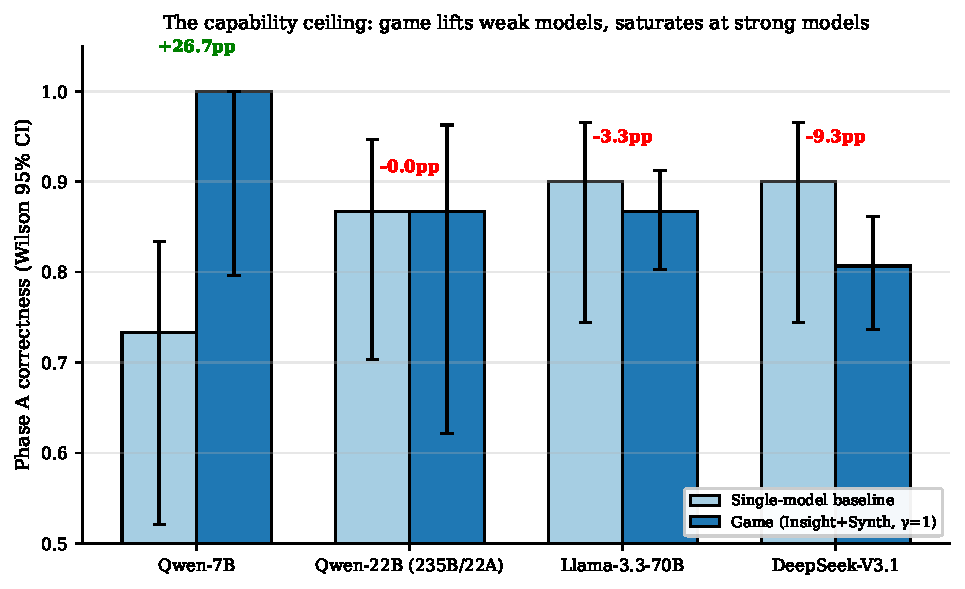
\includegraphics[width=0.85\linewidth]{figures/fig8_capability_ceiling.pdf}
\caption{The capability ceiling.
For each of four base models, the single-model Phase~A baseline is shown alongside the corresponding $4$-agent \textsc{Insight+Synth} game at $\g\!=\!1$.
Cheap models (\texttt{qwen-7b} at $73\%$) are lifted substantially; strong models (\texttt{llama-70b} and \texttt{deepseek-v3.1}, both at $90\%$ baseline) are not lifted.
Wilson $95\%$ CIs shown.}
\label{fig:ceiling}
\end{figure}

\begin{table}[h]
\centering\small
\caption{Family replication: the synthesis-completed game on three model families with different baseline strengths.}
\label{tab:ceiling}
\begin{tabular}{lcccc}
\toprule
Base model & Single baseline & Game (Insight+Synth, $\g\!=\!1$) & $\Delta$ \\
\midrule
\texttt{qwen-7b}        & $73.3\%$ ($22/30$) & $\mathbf{100.0\%}$ ($15/15$, main sweep) & $\mathbf{+26.7}$pp \\
\texttt{qwen-22b}       & $86.7\%$ ($26/30$) & $93.3\%$ ($14/15$, main sweep)           & $+6.6$pp \\
\texttt{llama-3.3-70b}  & $90.0\%$ ($27/30$) & $86.7\%$ ($130/150$)                     & $-3.3$pp \\
\texttt{deepseek-v3.1}  & $90.0\%$ ($27/30$) & $80.7\%$ ($121/150$)                     & $-9.3$pp \\
\bottomrule
\end{tabular}
\end{table}

The pattern is consistent: \textbf{the magnitude of the game's lift is monotonic in the gap between the single-model baseline and the achievable ceiling}.

\subsection{Cost--performance Pareto frontier}\label{app:pareto}

\begin{table}[h]
\centering\small
\caption{Cheapest collective configurations achieving $100\%$ correctness on Phase~A ($n = 15$ episodes per condition), compared to single-model baselines including the corrected frontier baseline. Cost-ratio column is relative to the corrected frontier.}
\label{tab:pareto}
\resizebox{\linewidth}{!}{%
\begin{tabular}{llcrr}
\toprule
Configuration & Correctness & Cost/prob & Ratio \\
\midrule
\multicolumn{4}{l}{\emph{Single-model references}} \\
\texttt{qwen-7b} (single) & $73.3\%$ & \$$0.00010$ & $1/46$ \\
\texttt{qwen-22b} (single) & $86.7\%$ & \$$0.00020$ & $1/23$ \\
\texttt{llama-3.3-70b} (single) & $90.0\%$ & \$$0.00027$ & $1/17$ \\
\texttt{qwen-17b} (thinking) & $86.7\%$ & \$$0.00461$ & $1\times$ (ref.) \\
\midrule
\multicolumn{4}{l}{\emph{Collectives achieving $100\%$ on Phase~A}} \\
\texttt{all-7b} $\times$ \textsc{Ins+Synth} ($\g\!=\!1$) & $100\%$ & \$$0.00025$ & $\mathbf{1/18}$ \\
\texttt{all-7b} $\times$ \textsc{Ins+Synth} ($\g\!=\!4$) & $100\%$ & \$$0.00031$ & $1/15$ \\
\texttt{p22b-c7b} $\times$ \textsc{Ins+Synth} ($\g\!=\!1$) & $100\%$ & \$$0.00044$ & $1/10$ \\
\texttt{p7b-s22b} $\times$ \textsc{Full Deb.} ($\g\!=\!0.5$) & $100\%$ & \$$0.00044$ & $1/10$ \\
\texttt{all-22b} $\times$ \textsc{Ins+Synth} ($\g\!=\!4$) & $100\%$ & \$$0.00047$ & $1/10$ \\
\texttt{all-22b} $\times$ \textsc{Full Deb.} ($\g\!=\!0.5$) & $100\%$ & \$$0.00066$ & $1/7$ \\
\bottomrule
\end{tabular}%
}
\end{table}

\subsection{Full ARC-AGI ranking}\label{app:arc-ranking}

\begin{figure}[h]
\centering
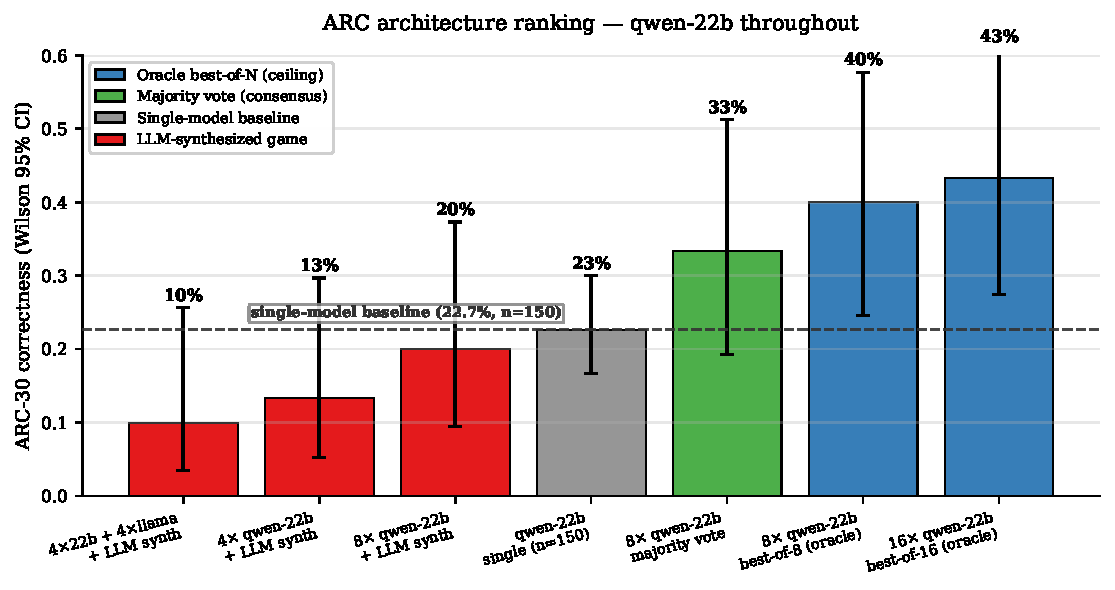
\includegraphics[width=0.95\linewidth]{figures/fig10_arc_ranking.pdf}
\caption{Seven architectures on ARC-AGI ($30$ problems, all using \texttt{qwen-22b} as the proposer; mixed-arch row uses $4$ \texttt{qwen-22b} + $4$ \texttt{llama-70b}).
Pure parallelism (oracle best-of-$N$, blue) reaches the natural ceiling of $40$--$43\%$.
Simple majority vote (green) captures $83\%$ of the oracle ceiling at $33.3\%$.
LLM-synthesized games (red) all fall \emph{below} the single-model baseline.
Wilson $95\%$ CIs shown.}
\label{fig:arc_ranking}
\end{figure}

\begin{table}[h]
\centering\small
\caption{Seven ARC-AGI architectures ranked by correctness ($30$ problems, $\texttt{qwen-22b}$ proposers throughout).}
\label{tab:arc}
\resizebox{\linewidth}{!}{%
\begin{tabular}{@{}lcccc@{}}
\toprule
Configuration & Rate & Wilson 95\% CI & \$/prob & $\Delta$ \\
\midrule
best-of-$16$ (oracle) & $\mathbf{43.3\%}$ \scriptsize($13/30$) & $[27.4, 60.8]$ & $0.017$ & $+20.7$ \\
best-of-$8$ (oracle) & $40.0\%$ \scriptsize($12/30$) & $[24.6, 57.7]$ & $0.008$ & $+17.3$ \\
\textbf{best-of-$8$ maj.\ vote} & $\mathbf{33.3\%}$ \scriptsize($10/30$) & $[19.2, 51.2]$ & $0.008$ & $\mathbf{+10.7}$ \\
\midrule
single-shot ($n\!=\!150$) & $22.7\%$ \scriptsize($34/150$) & $[16.7, 30.0]$ & $0.001$ & --- \\
\midrule
$8\!\times$ + LLM synth & $20.0\%$ \scriptsize($6/30$) & $[9.5, 37.3]$ & $0.010$ & $-2.7$ \\
$4\!\times$ + LLM synth & $13.3\%$ \scriptsize($4/30$) & $[5.3, 29.7]$ & $0.006$ & $-9.4$ \\
$4\!\times$\texttt{22b}+$4\!\times$\texttt{llama} + synth & $10.0\%$ \scriptsize($3/30$) & $[3.5, 25.6]$ & $0.015$ & $-12.7$ \\
\bottomrule
\end{tabular}%
}
\end{table}

%% ====================================================================
\section{Symbolic Verification: Additional Details}\label{app:symver-details}
%% ====================================================================

This appendix provides failure analysis and replication details for the symbolic verification experiments in Section~\ref{sec:act2}.

\subsection{AIME failure analysis}

Of the $7$ incorrect AIME~2024 problems: $5$ produced no runnable code at all (all $16$ samples errored or timed out, predominantly on higher-numbered problems); $2$ produced runnable code that computed the wrong integer.
Some correct answers had very low run-success rates (e.g., I-14 had only $1/16$ samples produce runnable code, but that single sample was correct).
The architecture is robust to high per-sample failure rates because majority vote only needs one correct sample in the pool.

\subsection{AIME 2025 replication}

To address the small-sample concern ($n\!=\!30$), we replicated on the $30$ problems from AIME~2025: $17/30 = 56.7\%$ (Wilson $[39.2\%, 72.6\%]$).
The combined AIME~2024+2025 rate is $40/60 = 66.7\%$ ($[54.0\%, 77.3\%]$), tightening the CI from $\pm 15$pp to $\pm 12$pp.
The drop from $76.7\%$ (2024) to $56.7\%$ (2025) reflects the harder problem distribution in AIME~2025.

\subsection{HumanEval metric caveat}

Our $97.0\%$ is pass@$K$ with $K\!=\!16$ and execution-based filtering: a problem is ``solved'' if \emph{any} of $16$ samples passes all unit tests.
The published frontier numbers (o1 at $93\%$, Claude at $92\%$, etc.) are typically reported as pass@$1$---a single attempt, no filtering.
Pass@$K$ with execution is a strictly easier metric than pass@$1$ without execution; any model's pass@$K$ is an upper bound on its pass@$1$.
The comparison is therefore \emph{not} apples-to-apples on the metric axis.
What \emph{is} apples-to-apples is the cost-per-correct comparison: our architecture uses $K\!=\!16$ samples and execution as its mechanism, and the total cost includes all $16$ calls.
A fair same-metric comparison would require running the frontier models at $K\!=\!16$ with the same execution filter---which we expect would also lift their pass rates, narrowing the accuracy gap while preserving the cost gap.

\subsection{ARC-AGI-1 verifiability boundary confirmation}

The same-task DeepSeek-V3.1 baseline ($n\!=\!400$) produces $2.8\%$ strict-grid-match on the evaluation split.
Manual inspection reveals that DeepSeek-V3.1 achieves $80$--$94\%$ cell-level match on most tasks---it ``almost'' solves them---but ARC's exact-grid scoring destroys near-correct outputs.
This is precisely the verifiability boundary in mechanistic form: the frontier model cannot self-verify its output to fix the last wrong cell, and it has no external feedback loop to catch the error.
Our architecture's program-execution filter catches these errors during candidate screening, which is why the architecture works despite using a weaker base model.

%% ====================================================================
\section{Null Result Details}\label{app:null-details}
%% ====================================================================

This appendix provides full details for the five null results summarized in Table~\ref{tab:six-nulls}.

\subsection{Null result: critic-driven refinement adds nothing}\label{app:critic}

We tested whether a more elaborate architecture---a critic that diagnoses specific execution failures and feeds structured feedback to the proposer for re-generation---could improve over the simple $K$-sample verifier loop.
On the same $30$-task ARC training battery, with matched total compute budget ($K_\text{initial}\!=\!16$ cold samples + $2$ rounds of $8$ critic-guided refinements = $32$ candidates per task, same as $K\!=\!32$ cold samples in the baseline):

\begin{center}\small
\begin{tabular}{lcc}
\toprule
Architecture & Deployable & Wilson 95\% CI \\
\midrule
$K\!=\!32$ cold samples (baseline) & $13/30 = 43.3\%$ & $[27.4\%, 60.8\%]$ \\
$K\!=\!16$ cold + $16$ critic refinements & $12/30 = 40.0\%$ & $[24.6\%, 57.7\%]$ \\
\bottomrule
\end{tabular}
\end{center}

The critic recovered exactly $1$ task across both refinement rounds ($\sim\!9\%$ critic success rate over $\sim\!88$ critic calls).

\subsection{Null result: ARC-AGI-2 breaks the architecture}\label{app:arc2}

ARC-AGI-2 (launched 2025) is materially harder than ARC-AGI-1; all published frontier models score below $5\%$.
We ran our architecture (identical configuration: \texttt{qwen-22b}, $K\!=\!16$, same Python DSL) on $100$ randomly sampled tasks from the ARC-AGI-2 test split.

Result: $0/100$ deployable (Wilson 95\% CI $[0.0\%, 3.7\%]$).
Only $1$ task in $100$ produced any program that passed all training pairs.

The diagnosis is clear: our $30$-primitive Python grid library \emph{cannot express} the higher-level conceptual abstractions that ARC-AGI-2 tests.
The boundary of the symbolic-verification approach is not verification quality---the sandbox executes perfectly---but \textbf{DSL coverage}: the proposer cannot write programs for transformations the DSL cannot represent.

\subsection{Null result: weak complementary proposers do not improve a strong one}\label{app:heterogeneous}

Three models (\texttt{qwen-22b}, DeepSeek-V3.1, Llama-3.3-70B) were each run at $K\!=\!8$ on the same $400$-task ARC-AGI-1 evaluation split.
On the $236$ tasks where all three models completed:

\begin{center}\small
\begin{tabular}{lccr}
\toprule
Configuration & $K$ total & Deployable & Rate \\
\midrule
\texttt{qwen-22b} alone & $8$ & $37/236$ & $15.7\%$ \\
\texttt{qwen-22b} alone (budget baseline) & $16$ & $41/236$ & $17.4\%$ \\
$3$-model union & $8{+}8{+}8{=}24$ & $39/236$ & $16.5\%$ \\
\bottomrule
\end{tabular}
\end{center}

The $3$-model union at $K\!=\!24$ \textbf{loses} to the budget-matched single-model baseline at $K\!=\!16$ ($16.5\%$ vs.\ $17.4\%$).
DeepSeek-V3.1 and Llama-70B are $\sim\!20\times$ worse than \texttt{qwen-22b} as ARC program proposers; they are not complementary specialists---they simply cannot write grid-transformation programs in our DSL.
This tests whether models with very low baseline capability add complementary coverage to a strong proposer, not whether model diversity in general is irrelevant.

\subsection{Null result: evolutionary refinement with inter-round information flow}\label{app:evolutionary}

Unlike the critic loop, this test uses full evolutionary context: the top-$3$ partial-pass programs from round $N$ are shown to proposers in round $N{+}1$ with per-pair pass/fail diagnostics and structural comparisons.
Three rounds of $K\!=\!8$ each (total $24$ candidates per task) on the same $30$-task ARC training battery:

\begin{center}\small
\begin{tabular}{lccc}
\toprule
Round & $K$ cumulative & Deployable & $\Delta$ vs.\ previous \\
\midrule
Round 1 (cold) & $8$ & $11/30$ ($36.7\%$) & --- \\
Round 2 (evolutionary) & $16$ & $12/30$ ($40.0\%$) & $+1$ task \\
Round 3 (evolutionary) & $24$ & $13/30$ ($43.3\%$) & $+1$ task \\
\midrule
Cold $K\!=\!8$ baseline & $8$ & $13/30$ ($43.3\%$) & --- \\
Cold $K\!=\!32$ baseline & $32$ & $13/30$ ($43.3\%$) & --- \\
\bottomrule
\end{tabular}
\end{center}

The evolutionary refinement recovers $+2$ tasks across rounds $2$--$3$, reaching $13/30 = 43.3\%$---\textbf{exactly tying} the cold $K\!=\!8$ baseline.
Inter-round information flow does not unlock solutions that cold sampling cannot reach.

%% ====================================================================
\section{Discussion: Additional Topics}\label{app:discussion-extra}
%% ====================================================================

This appendix collects discussion topics omitted from the main body for space.

\subsection{Adding a game framework does not appear to improve over simple selection}\label{app:game-remark}

We initially conjectured that a mean-field-game-style congestion mechanism, with informative value priors over reasoning frameworks, would outperform simpler unaware allocators because it concentrates agents on high-value frameworks while preserving coverage of low-value ones.
The mechanism does behave as theory predicts: the diversity metric responds cleanly to the congestion parameter ($D=0.46 \to 0.75$ at $\g\!=\!0.5$), and the value-aware variant preferentially places agents on high-value frameworks ($\sim 62\%$ vs $\sim 50\%$ for random in the $N\!=\!32$ test).
But across two fundamentally different regimes ($N\!<\!K$ and $N\!\gg\!K$, $1{,}350$ episodes total), the value-aware mechanism is statistically indistinguishable from random selection and round-robin (all pairwise $p > 0.4$, see Section~\ref{sec:results-falsification}).

Our reading of this finding is that \textbf{adding a game-theoretic framework on top of a strong synthesizer does not appear to add measurable value on the task class we study.}
The synthesizer does the recognition work; the framework distribution it receives is a second-order detail.
The practical recommendation is therefore: do not invest in elaborate framework selection mechanisms. Use a deterministic round-robin or random selection over a curated set of high-quality reasoning frameworks; spend your engineering effort on the synthesizer and on the framework definitions themselves.

\subsection{Why the original frontier baseline was misleading}\label{app:frontier}

The original main-sweep \texttt{qwen-17b} baseline used the Together AI \texttt{/no\_think} mode with a $1024$-token output budget---a configuration that suppresses the model's intended chain-of-thought and forces it to answer directly.
We adopted this configuration to control for the cost of thinking tokens during the main sweep, but the Tier 1.4 re-run shows it produced an unfair comparison.
With thinking enabled and a $4096$-token budget, \texttt{qwen-17b} jumps from $70\%$ to $86.7\%$ on Phase~A and from $80\%$ to $90\%$ on GSM8K-$50$.

The lesson generalizes beyond this specific experiment.
Frontier reasoning models are designed to be deployed with their thinking budget available; benchmarking them without that budget produces a misleading impression of their cost-performance position.
The cost-ratio claim of this paper now uses the corrected baseline (\$$0.00461$ per problem at $86.7\%$) and reports an $18\times$ ratio---down from the original $23\times$ but still substantial and fairer.

\subsection{The verifiability boundary, refined}\label{app:why-verifiability}

The capability ceiling is one boundary; the verifiability boundary is the other, and it has a more fundamental character.
The capability ceiling says \emph{when} the synthesis effect saturates; the verifiability boundary says \emph{whether} the mechanism even has the right sign.

The ARC reversal forces a refinement of the recognition story.
On Phase~A and GSM8K, the synthesizer's recognition accuracy $p_{\rm synth}^\star$ is high because the LLM can verify a candidate answer cheaply: re-read the question, re-do the arithmetic, check that the candidate matches.
On ARC, the verification path is broken: to check whether a candidate output grid is correct, the LLM would have to re-derive the underlying transformation rule from the training input--output pairs, then apply it to the test input, then compare to the candidate.
\emph{Re-deriving the transformation is the original problem.}

This generates a falsifiable prediction.
Define the verification cost $V(\text{task})$ as the marginal compute the synthesizer must spend to verify a candidate, beyond the cost of reading it.
On Phase~A and GSM8K, $V$ is low.
On ARC, $V$ is approximately equal to the cost of solving the problem from scratch.
The synthesis effect is positive when $V$ is low and negative when $V$ approaches the generation cost.
This suggests two empirically testable corollaries: (1)~on ARC the right architecture is one that supplies an \emph{external} verifier the LLM can defer to; (2)~the synthesis effect should reverse on any task where verification requires re-deriving the problem, not just visual-spatial ones.

\subsection{Threats to validity}\label{app:threats}

\paragraph{Task battery scope.}
The Phase~A battery is hand-constructed and elementary by design; GSM8K and ARC-AGI extend the test to two standard public benchmarks with very different output structures.
This three-domain coverage establishes the verifiability boundary as more than a Phase-A artifact, but the boundary needs replication across more domains to become a robust criterion.
MATH \cite{Hendrycks2021MATH} (verifiable), HumanEval \cite{Chen2021HumanEval} (verifiable via execution), MuSR \cite{Sprague2024MuSR} (multi-step reasoning, marginal verifiability), and 3D spatial reasoning benchmarks (non-verifiable) are the natural next targets.

\paragraph{Synthesis aggregator confound.}
The Tier 1.2 ablation establishes that LLM aggregation---not reasoning content---is the dominant active ingredient.
This refines but does not eliminate a residual concern: a more sophisticated unlearned aggregator (e.g., trust-weighted vote, or self-consistency-style entropy weighting) might recover much of the synthesis effect without the LLM call.

\paragraph{Capability-ceiling generalization.}
Our family-replication result shows that two strong base models (Llama-70B and DeepSeek-V3.1) at $90\%$ Phase~A baseline do not benefit from the game.
This is consistent with the capability-ceiling story but does not establish it as a universal property.

\paragraph{DSL as domain engineering.}
The symbolic-verification architecture requires a task-specific representation language: a $30$-primitive Python grid library for ARC-AGI, a \texttt{sympy}-enabled sandbox for AIME, and a unit-test execution environment for HumanEval.
This is non-trivial domain engineering---the ``no fine-tuning, no PRM'' framing slightly understates the supervision involved.
The ARC-AGI-2 null result ($0/100$) exposes this limit directly.

\paragraph{Prompt sensitivity.}
All experiments use a single prompt template per task type.
We have not systematically varied prompts; it is possible that prompt design interacts with the synthesis-vs-majority-vote comparison.
Model version drift is also a concern: all Together~AI experiments were conducted over a two-week window (April 2026) against serverless endpoints whose underlying weights could in principle change.
We release exact model identifiers and all prompts in the code repository.

\paragraph{Statistical power.}
The main-sweep per-condition CIs are wide ($\pm 8$--$15$pp at $n = 15$).
The aggregate findings (topology effect, $\g$ saturation) are based on $n \approx 450$ per topology and have non-overlapping CIs.
Per-cell findings should be interpreted as suggestive rather than as significance tests.

\subsection{Future work}\label{app:future}

\paragraph{Learned verifiers for non-verifiable tasks.}
Our Section~\ref{sec:act2} results show that symbolic verification dissolves the verifiability boundary.
The natural next question is whether \emph{learned} verifiers---process reward models (PRMs) trained on ground-truth trajectories \cite{Lightman2023PRM}---can play the same role on tasks without natural symbolic verification.

\paragraph{Replication of the verifiability boundary on more domains.}
Replicating the boundary on additional domains would strengthen the predictive criterion: long-form structured generation, multi-step planning, complex code that requires execution to verify, and 3D spatial layouts are all natural candidates.

\paragraph{Unlearned aggregators.}
An open question is whether more sophisticated unlearned aggregators (trust-weighted vote, self-consistency entropy weighting, learned ranking) can recover most of the LLM-aggregator gain at lower cost.

\paragraph{Tiered escalation.}
A tiered system would start at the cheapest model, escalate to larger models when verification fails, and could substantially improve cost efficiency on heterogeneous task distributions.

\paragraph{The capability ceiling formalized.}
A tighter characterization---ideally, an explicit formula relating $p_{\rm synth}^\star$ to measurable model properties---would convert the boundary from a deployment heuristic into a quantitative prediction.

%% ====================================================================
% BIBLIOGRAPHY
%% ====================================================================
\begin{thebibliography}{99}

\bibitem{Wei2022CoT}
J.~Wei, X.~Wang, D.~Schuurmans, M.~Bosma, B.~Ichter, F.~Xia, E.~Chi, Q.~Le, and D.~Zhou.
\newblock Chain-of-thought prompting elicits reasoning in large language models.
\newblock In \emph{NeurIPS}, 2022.

\bibitem{Wang2023SelfConsistency}
X.~Wang, J.~Wei, D.~Schuurmans, Q.~Le, E.~Chi, S.~Narang, A.~Chowdhery, and D.~Zhou.
\newblock Self-consistency improves chain-of-thought reasoning in language models.
\newblock In \emph{ICLR}, 2023.

\bibitem{Yao2023ToT}
S.~Yao, D.~Yu, J.~Zhao, I.~Shafran, T.~L.~Griffiths, Y.~Cao, and K.~Narasimhan.
\newblock Tree of thoughts: Deliberate problem solving with large language models.
\newblock \emph{arXiv:2305.10601}, 2023.

\bibitem{Besta2024GoT}
M.~Besta, N.~Blach, A.~Kubicek, R.~Gerstenberger, L.~Gianinazzi, et~al.
\newblock Graph of thoughts: Solving elaborate problems with large language models.
\newblock In \emph{Proc.\ AAAI}, 2024.

\bibitem{Wu2023AutoGen}
Q.~Wu, G.~Bansal, J.~Zhang, Y.~Wu, B.~Li, E.~Zhu, L.~Jiang, X.~Zhang, S.~Zhang, J.~Liu, A.~H.~Awadallah, R.~W.~White, D.~Burger, and C.~Wang.
\newblock {AutoGen}: Enabling next-gen {LLM} applications via multi-agent conversation.
\newblock \emph{arXiv:2308.08155}, 2023.

\bibitem{Hong2024MetaGPT}
S.~Hong, M.~Zhuge, J.~Chen, X.~Zheng, Y.~Cheng, C.~Zhang, et~al.
\newblock {MetaGPT}: Meta programming for a multi-agent collaborative framework.
\newblock In \emph{ICLR}, 2024.

\bibitem{Li2023CAMEL}
G.~Li, H.~A.~A.~K.~Hammoud, H.~Itani, D.~Khizbullin, and B.~Ghanem.
\newblock {CAMEL}: Communicative agents for ``mind'' exploration of large language model society.
\newblock In \emph{NeurIPS}, 2023.

\bibitem{Qian2024ChatDev}
C.~Qian, W.~Liu, H.~Liu, N.~Chen, Y.~Dang, J.~Li, et~al.
\newblock {ChatDev}: Communicative agents for software development.
\newblock In \emph{Proc.\ ACL}, 2024.

\bibitem{Irving2018Debate}
G.~Irving, P.~Christiano, and D.~Amodei.
\newblock {AI} safety via debate.
\newblock \emph{arXiv:1805.00899}, 2018.

\bibitem{Du2023Debate}
Y.~Du, S.~Li, A.~Torralba, J.~B.~Tenenbaum, and I.~Mordatch.
\newblock Improving factuality and reasoning in language models through multiagent debate.
\newblock \emph{arXiv:2305.14325}, 2023.

\bibitem{Khan2024Debate}
A.~Khan, J.~Hughes, D.~Valentine, L.~Ruis, K.~Sachan, A.~Raghavan, et~al.
\newblock Debating with more persuasive {LLMs} leads to more truthful answers.
\newblock In \emph{ICML}, 2024.

\bibitem{Shinn2023Reflexion}
N.~Shinn, F.~Cassano, A.~Gopinath, K.~Narasimhan, and S.~Yao.
\newblock Reflexion: Language agents with verbal reinforcement learning.
\newblock In \emph{NeurIPS}, 2023.

\bibitem{Madaan2023SelfRefine}
A.~Madaan, N.~Tandon, P.~Gupta, S.~Hallinan, L.~Gao, S.~Wiegreffe, et~al.
\newblock Self-{R}efine: Iterative refinement with self-feedback.
\newblock In \emph{NeurIPS}, 2023.

\bibitem{Shazeer2017MoE}
N.~Shazeer, A.~Mirhoseini, K.~Maziarz, A.~Davis, Q.~Le, G.~Hinton, and J.~Dean.
\newblock Outrageously large neural networks: The sparsely-gated mixture-of-experts layer.
\newblock In \emph{ICLR}, 2017.

\bibitem{Leviathan2023Speculative}
Y.~Leviathan, M.~Kalman, and Y.~Matias.
\newblock Fast inference from transformers via speculative decoding.
\newblock In \emph{ICML}, 2023.

\bibitem{Cobbe2021GSM8K}
K.~Cobbe, V.~Kosaraju, M.~Bavarian, M.~Chen, H.~Jun, L.~Kaiser, et~al.
\newblock Training verifiers to solve math word problems.
\newblock \emph{arXiv:2110.14168}, 2021.

\bibitem{Hendrycks2021MATH}
D.~Hendrycks, C.~Burns, S.~Kadavath, A.~Arora, S.~Basart, E.~Tang, D.~Song, and J.~Steinhardt.
\newblock Measuring mathematical problem solving with the {MATH} dataset.
\newblock In \emph{NeurIPS Datasets and Benchmarks}, 2021.

\bibitem{Sprague2024MuSR}
Z.~Sprague, F.~Yin, J.~D.~Rodriguez, D.~Jiang, M.~Wadhwa, P.~Singhal, X.~Zhao, X.~Ye, K.~Mahowald, and G.~Durrett.
\newblock {MuSR}: Testing the limits of chain-of-thought with multistep soft reasoning.
\newblock In \emph{ICLR}, 2024.

\bibitem{Chollet2019ARC}
F.~Chollet.
\newblock On the measure of intelligence.
\newblock \emph{arXiv:1911.01547}, 2019.

\bibitem{LasryLions2007}
J.-M.~Lasry and P.-L.~Lions.
\newblock Mean field games.
\newblock \emph{Japanese Journal of Mathematics}, 2(1):229--260, 2007.

\bibitem{HuangMalhameCaines2006}
M.~Huang, R.~P.~Malham\'e, and P.~E.~Caines.
\newblock Large population stochastic dynamic games: closed-loop {McKean--Vlasov} systems and the {Nash} certainty equivalence principle.
\newblock \emph{Communications in Information and Systems}, 6(3):221--252, 2006.

\bibitem{Gomes2010}
D.~A.~Gomes, J.~Mohr, and R.~R.~Souza.
\newblock Discrete time, finite state space mean field games.
\newblock \emph{Journal de Math\'ematiques Pures et Appliqu\'ees}, 93(2):308--328, 2010.

\bibitem{Gueant2015}
O.~Gu\'eant.
\newblock Existence and uniqueness result for mean field games with congestion effect on graphs.
\newblock \emph{Applied Mathematics \& Optimization}, 72(2):291--303, 2015.

\bibitem{Cecchin2019}
A.~Cecchin and G.~Pelino.
\newblock Convergence, fluctuations and large deviations for finite state mean field games.
\newblock \emph{Stochastic Processes and their Applications}, 129(11):4510--4555, 2019.

\bibitem{CarmonaDelarue2018}
R.~Carmona and F.~Delarue.
\newblock \emph{Probabilistic Theory of Mean Field Games with Applications}, volume 83--84 of \emph{Probability Theory and Stochastic Modelling}.
\newblock Springer, 2018.

\bibitem{Achdou2020MFGTraffic}
Y.~Achdou, P.~Cardaliaguet, F.~Delarue, A.~Porretta, and F.~Santambrogio.
\newblock \emph{Mean Field Games}, volume 2281 of \emph{Lecture Notes in Mathematics}.
\newblock Springer, 2020.

\bibitem{Lachapelle2011MFGCrowd}
A.~Lachapelle and M.-T.~Wolfram.
\newblock On a mean field game approach modeling congestion and aversion in pedestrian crowds.
\newblock \emph{Transportation Research Part B}, 45(10):1572--1589, 2011.

\bibitem{Wilson1927}
E.~B.~Wilson.
\newblock Probable inference, the law of succession, and statistical inference.
\newblock \emph{Journal of the American Statistical Association}, 22(158):209--212, 1927.

%% -- Act II references --

\bibitem{Li2022AlphaCode}
Y.~Li, D.~Choi, J.~Chung, N.~Kushman, J.~Schrittwieser, et~al.
\newblock Competition-level code generation with AlphaCode.
\newblock \emph{Science}, 378(6624):1092--1097, 2022.

\bibitem{RomeraParedes2024FunSearch}
B.~Romera-Paredes, M.~Barekatain, A.~Novikov, M.~Balog, M.~P.~Kumar, et~al.
\newblock Mathematical discoveries from program search with large language models.
\newblock \emph{Nature}, 625:468--475, 2024.

\bibitem{Snell2024ComputeOptimalTTS}
C.~Snell, J.~Lee, K.~Xu, A.~Kumar.
\newblock Scaling LLM test-time compute optimally can be more effective than scaling model parameters.
\newblock \emph{arXiv preprint arXiv:2408.03314}, 2024.

\bibitem{Liu2025Can1BSurpass405B}
Z.~Liu, Z.~Gou, Y.~Yang, H.~Peng, J.~Wang.
\newblock Can 1B LLM surpass 405B? Rethinking compute-optimal test-time scaling.
\newblock In \emph{ICLR}, 2025. arXiv:2502.06703.

\bibitem{ARCPrize2024Report}
F.~Chollet, M.~Knoop, G.~Kamradt.
\newblock ARC Prize 2024: Technical report.
\newblock \emph{arXiv preprint arXiv:2412.04604}, 2024.

\bibitem{Akyurek2024TTT}
E.~Aky\"urek, B.~Damani, L.~H.~Peng, A.~Sharma, S.~R.~Bowman, et~al.
\newblock The surprising effectiveness of test-time training for abstract reasoning.
\newblock \emph{arXiv preprint arXiv:2411.07279}, 2024.

\bibitem{Zhang2025StopOvervaluingMAD}
Y.~Zhang, Y.~Du, H.~Zhao.
\newblock Stop overvaluing multi-agent debate: We must rethink evaluation and embrace model heterogeneity.
\newblock In \emph{NeurIPS}, 2025. arXiv:2502.08788.

\bibitem{Chen2021HumanEval}
M.~Chen, J.~Tworek, H.~Jun, Q.~Yuan, et~al.
\newblock Evaluating large language models trained on code.
\newblock \emph{arXiv preprint arXiv:2107.03374}, 2021.

\bibitem{Saunders2022SelfCritique}
W.~Saunders, C.~Yeh, J.~Wu, S.~Bills, L.~Ouyang, J.~Ward, J.~Leike.
\newblock Self-critiquing models for assisting human evaluators.
\newblock \emph{arXiv preprint arXiv:2206.05802}, 2022.

\bibitem{Huang2023SelfCorrection}
J.~Huang, S.~S.~Gu, L.~Hou, Y.~Wu, X.~Wang, H.~Yu, J.~Han.
\newblock Large language models cannot self-correct reasoning yet.
\newblock In \emph{ICLR}, 2024. arXiv:2310.01798.

\bibitem{Kamoi2024SelfEval}
R.~Kamoi, Y.~Raman, Y.~Zhang, J.~Liu, R.~Balachandran.
\newblock When can LLMs actually correct their own mistakes? A critical survey of self-correction of LLMs.
\newblock \emph{Transactions of the ACL}, 2024. arXiv:2406.01297.

\bibitem{Lightman2023PRM}
H.~Lightman, V.~Kosaraju, Y.~Burda, H.~Edwards, B.~Baker, T.~Lee, J.~Leike, J.~Schulman, I.~Sutskever, K.~Cobbe.
\newblock Let's verify step by step.
\newblock In \emph{ICLR}, 2024. arXiv:2305.20050.

\end{thebibliography}

\end{document}
